\documentclass[iicol,lineno]{sn-jnl}


%%% PREAMBLE %%%
\usepackage[utf8]{inputenc}
\usepackage[T1]{fontenc}
\usepackage{lmodern}
%\usepackage[hidelinks]{hyperref}
\usepackage{diagbox}
\usepackage{todonotes}
\usepackage{ltl}
\usepackage{amssymb}
\usepackage{amsmath}
%\usepackage{amsthm}
\usepackage{stmaryrd}
\usepackage{tikz}
\usepackage{xcolor}
\usetikzlibrary{backgrounds, positioning, arrows, calc}
\usepackage{mathtools}
%\usepackage[linesnumbered,vlined,noend, ruled]{algorithm2e}
\usepackage[inline]{enumitem}  
\usepackage{cleveref}
\usepackage{lineno}
\usepackage{multirow}
\usepackage{wrapfig}
\usepackage[font=small]{caption}
\usepackage{subcaption}
%\linenumbers
\usepackage{hyperref}


\usepackage{graphicx}
\usepackage{amsfonts}%
\usepackage{mathrsfs}%
%\usepackage[title]{appendix}%
%\usepackage{textcomp}%
%\usepackage{manyfoot}%
%\usepackage{booktabs}%
%\usepackage{algorithm}%
%\usepackage{algorithmicx}%
%\usepackage{algpseudocode}%
%\usepackage{listings}%

%\usepackage{SpringerLarge}  % adjusts font sizing to the journal’s specs


\hypersetup{%
	%hidelinks,                % uncomment to use black links
	colorlinks=true,           % use colored links
	allcolors=blue!70!black,   % use dark blue for all links
	pdfstartview=Fit,          % open PDF viewer with side-pane hidden.
	breaklinks=true,
	% PDF metadata:
	%	pdfauthor={Borzoo, Anik, Dejan, Ege},
	%	pdftitle={{Approximate Distributed Monitoring under Partial Synchrony}}
}

%%% Save the class definition of \subparagraph
%\let\llncssubparagraph\subparagraph
%%% Provide a definition to \subparagraph to keep titlesec happy
%\let\subparagraph\paragraph
%%% Load titlesec
%\usepackage[compact]{titlesec}
%%% Revert \subparagraph to the llncs definition
%\let\subparagraph\llncssubparagraph

%%% MACROS %%%
\renewcommand{\cref}{\Cref}


% ----- DEBUG
\newcommand{\anik}[1]{\textcolor{orange}{\bf Anik: #1}}
\newcommand{\borzoo}[1]{\textcolor{purple}{\bf Borzoo: #1}}
\newcommand{\dejan}[1]{\textcolor{cyan!70!black}{\bf Dejan: #1}}
\newcommand{\ege}[1]{\textcolor{green!70!black}{\bf Ege: #1}}

\newcommand{\noteitem}{\ensuremath{\;{\bullet}\;}}
\setlength{\marginparwidth}{4.2cm}
\setlength{\marginparsep}{0.3cm}

\newcommand{\answer}[1]{{\color{white}#1}}
\newcommand{\orangenote}[2][]{{\todo[color=orange!80,size=\footnotesize,#1]{\normalcolor\normalfont#2}}}
\newcommand{\bluenote}[2][]{{\todo[color=cyan!80,size=\footnotesize,#1]{\normalcolor\normalfont#2}}}
\newcommand{\greennote}[2][]{{\todo[color=green!80!black,size=\footnotesize,#1]{\normalcolor\normalfont#2}}}
\newcommand{\rednote}[2][]{{\todo[color=magenta!30,size=\footnotesize,#1]{\normalcolor\normalfont#2}}}
\newcommand\alert[1]{\textcolor{red}{#1}}
\newcommand\TODO{\textcolor{red}{TODO}}

\renewcommand{\pfx}{\textsf{prefix}}
\newcommand{\first}{\textsf{first}}
\newcommand{\last}{\textsf{last}}
\renewcommand{\sfx}{\textsf{suffix}}
\newcommand{\infx}{\textsf{infix}}
\newcommand{\conjunction}{\textsf{conj}}

\newcommand{\hb}{\rightsquigarrow}
\newcommand{\A}{\mathbb{A}}
\renewcommand{\S}{\mathbb{S}}
\newcommand{\fr}{\mathsf{fr}}
\newcommand{\CC}{\mathbb{C}}
\newcommand{\tr}{\mathsf{Tr}}
\newcommand{\AP}{\mathsf{AP}}
\newcommand{\true}{\texttt{true}}
\newcommand{\false}{\texttt{false}}
\newcommand{\CCF}{\mathsf{CCF}}
\newcommand{\ccf}{\mathsf{ccf}}
\newcommand{\destutter}{\mathsf{destutter}}
\newcommand{\stutter}{\mathsf{stutter}}
\newcommand*\BitAnd{\mathbin{\&}}
\newcommand*\BitOr{\mathbin{|}}
\newcommand*\ShiftLeft{\ll}
\newcommand*\ShiftRight{\gg}
\newcommand*\BitNeg{\ensuremath{\mathord{\sim}}}

\newcounter{resq}[section]
\newenvironment{resq}[1][]{%
	\refstepcounter{resq}%
	\par\medskip
	\noindent \textbf{RQ\theresq.}~\textit{#1} \rmfamily}{\medskip}
\newcommand{\thisquestion}{RQ\theresq\xspace}
\newcommand{\prevquestion}{RQ\the\numexpr\value{resq}-1\relax\xspace}

% ----- FIGURES
\tikzstyle{state}=[thick,minimum size=18pt, circle,draw]
\tikzstyle{transition}=[->,thick,>=stealth,shorten >=1pt,shorten <=1pt]
\tikzstyle{final}=[after node path={ node[state, scale=.8] at (\tikzlastnode) {} }]
\tikzstyle{initial}=[after node path={
	[to path={[transition] (\tikztostart) -- (\tikztotarget)}]
	(\tikzlastnode)++(180:22pt) edge (\tikzlastnode)
}]
\tikzset{
	bg/.default={},
	bg/.style={execute at end picture={
			\begin{scope}[on background layer]
				\node[xshift=-1mm, yshift=-1mm] (sw) at (current bounding box.south west) {};
				\node[xshift=1mm, yshift=1mm] (ne) at (current bounding box.north east) {};
				\node[xshift=1mm, yshift=-1mm] (nw) at (current bounding box.north west) {};
				\fill[fill=black!10,rounded corners] (sw) rectangle (ne);
				
				\ifx&#1&\else
				\node[anchor=north east, xshift=2pt] at (nw) {#1};
				\fi
			\end{scope}
	}},
}

% ----- NUMERICAL SETS
\newcommand{\Z}{\mathbb{Z}}
\newcommand{\ZZ}{\overline{\ref{ex:minresp}Z}}
\newcommand{\N}{\mathbb{N}}
\newcommand{\NN}{\overline{\N}}
\newcommand{\R}{\mathbb{R}}
\newcommand{\RR}{\R^{\pm \infty}}
\newcommand{\Q}{\mathbb{Q}}
\newcommand{\D}{\mathbb{D}}
\newcommand{\B}{\mathbb{B}}

% ------ FUNCTIONS
\newcommand{\avg}{\text{\normalfont avg}}
\newcommand{\disc}{\text{\normalfont disc}}
\newcommand{\fin}{\text{\normalfont fin}} 
\newcommand{\limavg}{\text{\normalfont limavg}} 

% ----- LTL SYNTAX
\renewcommand{\LTLf}{\LTLdiamond}
\let\LTLfinally\LTLf
\let\LTLeventually\LTLf
\renewcommand{\LTLg}{\LTLsquare}
\let\LTLalways\LTLg
\let\LTLglobally\LTLg
\renewcommand{\LTLo}{\LTLcircle}
\let\LTLnext\LTLo
\def\until{\kern.1em\mathcal{U}}
\def\since{\kern.1em\mathcal{S}}
%\newcommand \until      {\mathbin{\mathcal{U}\kern-.1em}}

\newcommand{\?}{\text{?}}

\newcommand{\req}{\texttt{rq}}
\newcommand{\ping}{\texttt{ping}}
\newcommand{\ack}{\texttt{ack}}
\newcommand{\gra}{\texttt{gr}}
\newcommand{\tick}{\texttt{tk}}
\newcommand{\other}{\texttt{oo}}
\newcommand{\off}{\texttt{off}}
%\newcommand{\ready}{\texttt{ready}}

% ----- MONITOR
\newcommand{\res}{\mathbf{r}}
\newcommand{\RES}{\mathbf{R}}
\newcommand{\ggeq}{\mathrel{\underline{\gg}}}
\newcommand{\lleq}{\mathrel{\underline{\ll}}}
\newcommand{\calM}{\mathcal{M}}
\newcommand{\calA}{\mathcal{A}}
\newcommand{\calB}{\mathcal{B}}
\newcommand{\prefixeq}{\preceq}
\newcommand{\prefix}{\prec}
\newcommand{\infPhi}{\inf\nolimits_\varPhi}
\newcommand{\supPhi}{\sup\nolimits_\varPhi}
\newcommand{\spec}{\textit{spec}}
\newcommand{\trace}{\textit{trace}}
\newcommand{\pref}{\textit{pref}}

% ----- GENERAL
\newcommand{\dom}[1]{{\textsf{dom}(#1)}}
\newcommand{\sem}[1]{{[\!\![#1]\!\!]}}
\newcommand{\suchthat}{\;\ifnum\currentgrouptype=16 \middle\fi|\;}
\let\st\suchthat
\newcommand{\defeq}{\coloneqq}
%\DeclarePairedDelimiter\floor{\lfloor}{\rfloor}
\newcommand\Circle[1][1.4]{\tikz[baseline=-3.3]{\draw(0,0)circle[radius=#1mm];}}

% ----- THEOREMS
%\newtheorem{observation}[theorem]{Fact}


\newtheorem{theorem}{Theorem}
\newtheorem{lemma}{Lemma}
\newtheorem{example}{Example}
\newtheorem{remark}{Remark}
\newtheorem{definition}{Definition}

\raggedbottom
%%\unnumbered% uncomment this for unnumbered level heads

\begin{document}
	\title[Approximate Distributed Monitoring under Partial Synchrony]{Approximate Distributed Monitoring under Partial Synchrony: Balancing Speed \& Accuracy}
	\author[1]{\fnm{Borzoo} \sur{Bonakdarpour}}\email{borzoo@msu.edu}
	\author[1]{\fnm{Anik} \sur{Momtaz}}\email{momtazan@msu.edu}
	\author[2]{\fnm{Dejan} \sur{Ni\v{c}kovi\'{c}}}\email{dejan.nickovic@ait.ac.at}
	\author*[3]{\fnm{N. Ege} \sur{Sara\c{c}}}\email{esarac@ista.ac.at}
	\affil[1]{\orgname{Michigan State University}}
	\affil[2]{\orgname{AIT Austrian Institute of Technology}}
	\affil*[3]{\orgname{Institute of Science and Technology Austria (ISTA)}}
	%%\pacs[JEL Classification]{D8, H51}
	%%\pacs[MSC Classification]{35A01, 65L10, 65L12, 65L20, 65L70}
	
	\maketitle
	
	\abstract{
		In distributed systems with processes that do not share a global clock, \emph{partial synchrony} is 
		achieved by clock synchronization 
		that guarantees bounded clock skew among all applications. Existing solutions for distributed 
		runtime verification under partial 
		synchrony against temporal logic specifications are exact but suffer from significant 
		computational overhead. In this paper, we propose an \emph{approximate} 
		distributed monitoring algorithm for Signal Temporal Logic (STL) that mitigates this issue by 
		abstracting away potential interleaving behaviors. 
		This conservative abstraction enables a significant speedup of the distributed monitors, albeit 
		with a tradeoff in accuracy. We address this 
		tradeoff with a methodology that combines our approximate monitor with its exact counterpart, 
		resulting in enhanced  
		efficiency without sacrificing precision. We evaluate our approach with multiple 
		experiments, 
		showcasing its efficacy in 
		both real-world applications and synthetic examples.
	}
	
	\keywords{distributed systems, approximate monitoring, partial synchrony}
	
	\section{Introduction} 
	\label{sec:introduction}
	
	\emph{Distributed systems} are networks of independent agents that work together to achieve a 
	common objective.
	%
	They come in many different forms.
	%
	For example, cloud computing uses distribution of resources and services over the internet to offer 
	to their users a scalable infrastructure with transparent on-demand access to computing power and 
	storage. 
	%
	Swarms of drones is another family of distributed systems where individual drones 
	collaborate to accomplish tasks like search and rescue or package delivery.
	%
	While each drone operates independently, it also communicates and coordinates with others to 
	successfully achieve their common objectives.
	%
	The individual agents in a distributed system typically do not share a global clock.
	%
	To coordinate actions across multiple agents, clock synchronization is often needed.
	%
	While perfect clock synchronization is impractical due to network latency and node failures, 
	algorithms such as the Network Time Protocol (NTP) allow agents to maintain a \emph{bounded 
		skew} between the synchronized clocks.
	%
	We then say that a distributed system has \emph{partial synchrony}. 
	
	Formal verification of distributed system is a notoriously hard problem, due to the combinatorial 
	explosion of all possible interleavings in the behaviors collected from individual agents.
	%
	% \emph{Runtime verification (RV)} provides a more pragmatic approach, in which a monitor observes 
	% a behavior of a distributed system and checks its correctness against a formal specification.
	\emph{Runtime verification (RV)} provides a more pragmatic approach in which a behavior of a distributed system is observed and its correctness is checked against a formal specification.
	%
	%\subsection{Motivation}
	%There has been emerging interest in designing RV techniques for distributed systems in the past few years.
	%
	We consider the \emph{distributed RV} setting where this task is performed by a single central monitor observing the independent agents (as opposed to \emph{decentralized RV} where the monitoring task itself is distributed).
	%
	Remotely related to the problem of distributed RV under partial synchrony are distributed RV in the 
	fully {\em synchronous}~\cite{ef20,cf16,bf16} and {\em 
		asynchronous}~\cite{cgnm13,mg05,og07,mb15,g20,bfrrt22} settings as well as  benchmarking 
	tools~\cite{aafi21} for assessing monitoring overhead.
	%
	The problem of distributed RV under partial synchrony assumption has been studied for Linear 
	Temporal Logic (LTL)~\cite{GangulyMB20} and Signal Temporal Logic (STL)~\cite{MomtazAB23} 
	specification languages.
	%
	The proposed solutions use Satisfiability-Modulo-Theory (SMT) solving to provide sound and 
	complete distributed monitoring procedures.
	%
	Although distributed RV monitors consume only a single distributed behavior at a time, this behavior 
	can have an excessive number of possible interleavings. 
	%
	Put another way, although RV deals only with the verification of a single execution at run time, it is 
	still prone to evaluating an explosion of combinations.
	%
	Hence, the exact distributed monitors from the literature can still suffer from significant 
	computational overhead.
	%
	This phenomenon has been observed even under partial synchrony~\cite{GangulyMB20,gmb24}, and becomes problematic even for offline monitoring of a large set of log files.
	
	%  \subsection{Contributions}
	
	To mitigate this issue, we propose a new approach for \emph{approximate} RV of STL 
	under partial synchrony.
	%
	In essence, we conservatively abstract away potential interleavings in distributed behaviors, resulting in their overapproximation.
	%
	This abstraction simplifies the representation of distributed behaviors into a set of Boolean 
	expressions, taking into account regions of uncertainty created by clock skews.
	%
	We define monitoring operations that evaluate temporal specifications over such expressions, 
	which result in monitoring verdicts on overapproximated behaviors.
	%
	This approximate solution yields an inevitable tradeoff between {\em accuracy} and {\em speedup}.
	%
	%That is,  gains in the monitoring speedup may result in reduced accuracy.
	%
	For applications where reduced accuracy is not acceptable, we devise a methodology that combines approximate and exact monitors, 
	with the aim to benefit from the enhanced efficiency without sacrificing 
	precision.
	%
	Approximate monitoring is also valuable in the sequential setting, with applications including
	monitoring with state estimation \cite{StollerBSGHSZ11,BartocciG13},
	quantitative monitoring and its resource-precision tradeoffs \cite{HenzingerS21,HenzingerMS22,HenzingerMS23},
	and various other uses \cite{AlechinaDL14,AcetoAFIL21}.
	
	
	
	We implemented our approach in a prototype tool and performed thorough evaluations on both 
	synthetic and real-world case studies (mutual separation in swarm of drones and a water distribution 
	system).
	%
	We first demonstrated that in many experiments, our approximate monitors achieve 
	speedups of up to 5 orders of magnitude compared to the exact SMT-based solution.
	%
	We empirically characterized the classes of specifications and behaviors for which our approximate 
	monitors achieve good precision.
	%
	%In our case studies, we observe up to 5 orders of magnitude speedup.
	%  (although in some cases the  improvement is not as much)
	%
	We finally showed that combining exact and approximate distributed RV yields significant efficiency gains on average without sacrificing precision, even with low-accuracy approximate monitors.
	
	%\paragraph{Organization.}
	%%\noindent\textit{Organization.}
	%Section~\ref{sec:preliminaries} presents the preliminary concepts.
	%%
	%Section~\ref{sec:semantics} introduces overapproximate semantics of STL while 
	%Sections~\ref{sec:approach} and~\ref{sec:algorithm} describe our approach in approximating traces 
	%and the associated monitoring algorithm, respectively.
	%%
	%We evaluate our approach in Section~\ref{sec:experiments}. Finally, we conclude in 
	%Section~\ref{sec:conclusion}.
	
	
	\section{Preliminaries} \label{sec:preliminaries}
	
	%We define boolean domain $\B = \{ \bot, \top \}$ as the set of boolean truth values, where $\bot < \top$ and they 
	%complement each other, i.e., $\overline{\bot} = \top$ and $\overline{\top} = \bot$.
	%
	We denote by $\B = \{ \top, \bot \}$ the set of Booleans, $\R$ the set of reals, $\R_{\geq 0}$ the set of nonnegative reals, and $\R_{> 0}$ the 
	set of positive reals.
	%
	An interval $I \subseteq \R$ of reals with the end points $a < b$ has length $|b-a|$.
	
	Let $\Sigma$ be a finite {\em alphabet}.
	%
	We denote by $\Sigma^*$ the set of finite words over $\Sigma$ and by $\epsilon$ the empty word.
	%
	For $u \in \Sigma^*$, we respectively write $\pfx(u)$ and $\sfx(u)$ for the sets of prefixes 
	and suffixes of $u$.
	%
	We also let $\infx(u) = \{v \in \Sigma^* \st \exists x,y \in \Sigma^* : u = xvy\}$.
	%
	For a nonempty word $u \in \Sigma^*$ and $1 \leq i \leq |u|$, we denote by $u[i]$ the $i$th letter of $u$.
	%, by $u[..i]$ the prefix of $u$ of length $i$, and by $u[i..]$ the suffix of $u$ of length $|u| - i + 1$. 
	%
	Given $u \in \Sigma^*$ and $\ell \geq 1$, we denote by $u^\ell$ the word obtained by concatenating $u$ by itself $\ell - 1$ times.
	Moreover, given $L \subseteq \Sigma^*$, we define $\first(L) = \{ u[1] \st u \in L\}$ and $\last(L) = \{ u[|u|] \st u \in L\}$
	For sets $L_1, L_2 \subseteq \Sigma^*$ of words, we let $L_1 \cdot L_2 = \{u \cdot v \st u \in L_1, v \in L_2\}$.
	For tuples $(u_1, \ldots, u_m)$ and $(v_1, \ldots, v_m)$ of words, we let $(u_1, \ldots, u_m) \cdot (v_1, \ldots, v_m) = (u_1 v_1, \ldots, u_m v_m)$.
	
	We define the function $\destutter : \Sigma^* \to \Sigma^*$ inductively.
	For all $\sigma \in \Sigma \cup \{\epsilon\}$, let $\destutter(\sigma) = \sigma$.
	For all $u \in \Sigma^*$ such that $u = \sigma_1 \sigma_2 v$ for some $\sigma_1,\sigma_2 \in 
	\Sigma$ and $v \in \Sigma^*$, we define it as follows:
	
	%\vspace{-1em}
	%\small
	\begin{equation*}
		\destutter(u) =
		\begin{cases}
			\destutter(\sigma_2 v) & \text{if } \sigma_1 = \sigma_2 \\
			\sigma_1 \cdot \destutter(\sigma_2 v) & \text{otherwise}
		\end{cases}
	\end{equation*}
	%\normalsize
	%For all $\sigma \in \Sigma \cup \{\epsilon\}$, let $\destutter(\sigma) = \sigma$.
	%%
	%For all $u \in \Sigma^*$ such that $u = \sigma_1 \sigma_2 v$ for some $\sigma_1,\sigma_2 \in 
	%\Sigma$ and $v \in \Sigma^*$, let (i) $\destutter(u) = \destutter(\sigma_2 v)$ if $\sigma_1 = 
	%\sigma_2$, and (ii) $\destutter(u) = \sigma_1 \cdot \destutter(\sigma_2 v)$ otherwise.
	%%
	For a set $L \subseteq \Sigma^*$ of finite words, we define $\destutter(L) = 
	\{\destutter(u) \st u \in L\}$.
	%
	We extend $\destutter$ to tuples of words in a synchronized manner: for all $\sigma \in \Sigma \cup \{\epsilon\}$  let $\destutter(\sigma, \ldots, \sigma) = (\sigma, \ldots, \sigma)$.
	Given a tuple $(u_1, \ldots, u_m) = (\sigma_{1,1} \sigma_{1,2} v_1, \ldots, \sigma_{m,1} \sigma_{m,2} v_m)$ of words of the same length, $\destutter(u_1, \ldots, u_m)$ is defined as expected:
	
	%\vspace{-1em}
	%\small
	\begin{align*}
		&\destutter(u_1, \ldots, u_m) = \\
		&\begin{cases}
			\destutter(\sigma_{1,2} v_1, \ldots, \sigma_{m,2} v_m) \text{ if $\sigma_{i,1} = \sigma_{i,2}$ for}\\ 
			\hspace{14em}\text{all $1 \leq i \leq m$} \\
			(\sigma_{1,1}, \ldots, \sigma_{m,1}) \cdot \destutter(\sigma_{1,2} v_1, \ldots, \sigma_{m,2} v_m) \\
			\hspace{15.5em}\text{otherwise}
		\end{cases}
	\end{align*}
	%\normalsize
	%Given a tuple $(u_1, \ldots, u_m) = (\sigma_{1,1} \sigma_{1,2} v_1, \ldots, \sigma_{m,1} \sigma_{m,2} v_m)$ of finite words of the same length, we define $\destutter(u_1, \ldots, u_m)$ as expected: (i) $\destutter(u_1, \ldots, u_m) = \destutter(\sigma_{1,2} v_1, \ldots, \sigma_{m,2} v_m)$ if $\sigma_{i,1} = 
	%\sigma_{i,2}$ for all $1 \leq i \leq m$, and (ii) $\destutter(u_1, \ldots, u_m) = (\sigma_{1,1}, \ldots, \sigma_{m,1}) \cdot \destutter(\sigma_{1,2} v_1, \ldots, \sigma_{m,2} v_m)$ otherwise.
	
	Moreover, given an integer $k \geq 0$, we define $\stutter_k : \Sigma^* \to \Sigma^*$ such that $\stutter_k(u) = \{v \in \Sigma^* \st |v| = k \land \destutter(v) = \destutter(u)\}$ if $k \geq |\destutter(u)|$, and $\stutter_k(u) = \emptyset$ otherwise.
	
	\paragraph*{Signal Temporal Logic (STL) \cite{MalerN13}.}
	%\noindent\textbf{Signal Temporal Logic (STL) \cite{MalerN13}.}
	Let $A,B \subset \R$.
	%
	A function $f : A \to B$ is
	\emph{right-continuous} iff $\lim_{a \to c^+} f(a) = f(c)$ for all $c \in A$, and
	%\emph{left-limited} iff $\lim_{a \to c^-} f(a) < \infty$ for all $c \in A$;
	\emph{non-Zeno} iff for every bounded interval $I \subseteq A$ there are finitely many $a \in I$ such that $f$ is not continuous at $a$.
	%
	A \emph{signal} is a right-continuous, non-Zeno, piecewise-constant function $x : [0,d) \to \R$ where $d \in \R_{> 0}$ is the duration of $x$ and $[0,d)$ is its temporal domain.
	Let $x : [0,d) \to \R$ be a signal.
	An \emph{event} of $x$ is a pair $(t, x(t))$ where $t \in [0,d)$.
	An \emph{edge} of $x$ is an event $(t, x(t))$ such that $\lim_{s \to t^-} x(s) \neq \lim_{s \to t^+} x(s)$.
	In particular, an edge is \emph{rising} if $\lim_{s \to t^-} x(s) < \lim_{s \to t^+} x(s)$, and it is \emph{falling} otherwise.
	A signal $x : [0,d) \to \R$ can be represented finitely by its initial value and edges: if $x$ has $m$ edges, then $x = (t_0, v_0) (t_1, v_1) \ldots (t_m, v_m)$ such that $t_0 = 0$, $t_{i-1} < t_i$, and $(t_i, v_i)$ is an edge of $x$ for all $1 \leq i \leq m$.
	
	\bgroup \color{red}
	Let $\AP$ be a set of \emph{atomic propositions}.
	The syntax of \emph{future STL} is given by the grammar $\varphi :=  p ~|~ \lnot \varphi ~|~ \varphi \land \varphi ~|~ \varphi \until_I \varphi$ and that of \emph{past STL} is given by $\varphi :=  p ~|~ \lnot \varphi ~|~ \varphi \land \varphi ~|~ \varphi \since_I \varphi$ where $p \in \AP$ and $I \subseteq \R_{\geq 0}$ is an interval.
	Below, when we speak of an STL formula, we mean either a future STL or a past STL formula.
	\egroup
	
	A \emph{trace} $w = (x_1, \ldots, x_n)$ is a finite vector of signals.
	We express atomic propositions as functions of trace values at a time point $t$,
	i.e., a proposition $p \in \AP$ over a trace $w = (x_1, \ldots, x_n)$ is defined as $f_p(x_1(t), \ldots, x_n(t)) > 0$ where $f_p : \R^n \to \R$ is a function.
	%i.e., a proposition $p \in \AP$ over a trace $w = (x_1, \ldots, x_n)$ is defined as $f_p(x_1(t), \ldots, x_n(t)) \sim_p c_p$ where $f_p : \R^n \to \R$ is a function, $c_p \in \R$ is a constant, and ${\sim_p} \in \{{<}, {\leq}, {\geq}, {>}\}$.
	Given intervals $I,J \subseteq \R_{\geq 0}$, we define $I \oplus J = \{i + j \st i \in I , j \in J\}$ and $I \ominus J = \{i - j \st i \in I , j \in J\}$, where we simply write $t$ for the singleton set $\{t\}$. 
	
	We recall the finite-trace qualitative semantics of STL defined over $\B$.
	Let $d \in \R_{> 0}$ and $w = (x_1, \ldots, x_n)$ with $x_i : [0,d) \to \R$ for all $1 \leq i \leq n$.
	Let $\varphi_1, \varphi_2$ be STL formulas and let $t \in [0,d)$.
	
	\bgroup \color{red}
	\begin{align*}
		(w,t) \models p \iff & f_p(x_1(t), \ldots, x_n(t)) > 0 \\
		(w,t) \models \lnot \varphi_1 \iff & \overline{(w,t) \models \varphi_1} \\
		(w,t) \models \varphi_1 \land \varphi_2 \iff & (w,t) \models \varphi_1 \land (w,t) \models \varphi_2 \\
		(w,t) \models \varphi_1 \until_I \varphi_2 \iff & \exists t' \in (t \oplus I) \cap [0,d) :  \\
		& (w,t') \models \varphi_2 \land \forall t'' \in (t, t') : \\
		& (w,t'') \models \varphi_1\\
		(w,t) \models \varphi_1 \since_I \varphi_2 \iff & \exists t' \in (t \ominus I) \cap [0,d) :  \\
		& (w,t') \models \varphi_2 \land \forall t'' \in (t', t) : \\
		& (w,t'') \models \varphi_1
	\end{align*}
	
	When $\varphi$ is a future (resp. past) STL formula, we simply write $w \models \varphi$ for $(w,0) \models \varphi$ (resp. $(w,d) \models \varphi$).
	We additionally use the following standard abbreviations: 
	$\false = p \land \lnot p$,
	$\true = \lnot \false$,
	$ \varphi_1 \lor \varphi_2 = \lnot (\lnot \varphi_1 \land \lnot \varphi_2)$,
	$\LTLf_I \varphi = \true \until_I \varphi$,
	$\LTLg_I \varphi = \lnot \LTLf_I \lnot \varphi$,
	$\LTLdiamondminus_I \varphi = \true \since_I \varphi$, and
	$\LTLsquareminus_I \varphi = \lnot \LTLdiamondminus_I \lnot \varphi$.
	Moreover, the untimed temporal operators are defined through their timed counterparts on the interval $[0,\infty)$.
	
	Future STL formulas whose timed operators are bounded (i.e., use of $\until_I$ is restricted to intervals $I$ with a real-valued right end point) can be translated to past STL formulas, which can be efficiently monitored online~\cite{MalerNP07,JaksicBGKNN15,Gol18}.
	\egroup
	
	\paragraph*{Distributed Semantics of STL \cite{MomtazAB23}.}
	%\noindent\textbf{Distributed Semantics of STL \cite{MomtazAB23}.}
	We consider an asynchronous and loosely-coupled message-passing system of $n \geq 2$ reliable agents producing a set of signals $x_1, \ldots, x_n$, where for some $d \in \R_{> 0}$ we have $x_i : [0,d) \to \R$ for all $1 \leq i \leq n$.
	%
	The agents do not share memory or a global clock.
	%
	Only to formalize statements, we speak of a \emph{hypothetical} global clock and denote its value by $T$.
	%
	For local time values, we use the lowercase letters $t$ and $s$.
	For a signal $x_i$, we denote by $V_i$ the set of its events, and by $E_i$ the set of its edges.
	%For a signal $x_i$, we denote by $V_i$ the set of its events, by $E_i^\uparrow$ the set of its rising edges, and by $E_i^\downarrow$ that of falling edges.
	%Moreover, we let $E_i = E_i^\uparrow \cup E_i^\downarrow$.
	%
	We represent the local clock of the $i$th agent as an increasing and divergent function $c_i : 
	\R_{\geq 0} \to \R_{\geq 0}$ that maps a global time $T$ to a local time $c_i(T)$.
	
	We assume that the system is \emph{partially synchronous}: the agents use a clock synchronization algorithm that guarantees a bounded clock skew with respect to the global clock, i.e., $|c_i(T) - c_j(T)| < \varepsilon$ for all $1 \leq i,j \leq N$ and $T \in \R_{\geq 0}$, where $\varepsilon \in \R_{> 0}$ is the maximum clock skew.
	
	\begin{definition} \label{defn:hb}
		A \emph{distributed signal} is a pair $(S, {\hb})$, where $S = (x_1, \ldots, x_n)$ is a vector of 
		signals and ${\hb}$ is the happened-before relation between events defined as follows:
		(1) For every agent, the events of its signals are totally ordered, i.e., for all $1 \leq i \leq n$ and all $(t, x_i(t)), (t', x_i(t')) \in V_i$, if $t < t'$ then $(t, x_i(t)) \hb (t', x_i(t'))$.
		(2) Every pair of events whose timestamps are at least $\varepsilon$ apart is totally ordered, i.e., for all $1 \leq i,j \leq n$ and all $(t, x_i(t)) \in V_i$ and $(t', x_j(t')) \in V_j$, if $t + \varepsilon \leq t'$ then $(t, x_i(t)) \hb (t', x_j(t'))$.
	\end{definition}
	
	The notion of \emph{consistent cut} captures possible global states.
	
	\begin{definition}
		Let $(S, {\hb})$ be a distributed signal of $n$ signals, and $V = \bigcup_{i = 1}^{n} V_i$ be the set of its events.
		A set $C \subseteq V$ is a \emph{consistent cut} iff for every event in $C$, all events that happened before  it also belong to $C$, i.e., for all $e, e' \in V$, if $e \in C$ and $e' \hb e$, then $e' \in C$.
	\end{definition}
	
	We denote by $\CC(T)$ the set of consistent cuts at global time $T$.
	Given a consistent cut $C$, its \emph{frontier} $\fr(C) \subseteq C$ is the set consisting of the last events in $C$ of each signal, i.e., $\fr(C) = \bigcup_{i = 1}^{n} \{ (t, x_i(t)) \in V_i \cap C \st \forall t' > t : (t', x_i(t')) \notin V_i \cap C \}$.
	
	\begin{definition}
		A \emph{consistent cut flow} is a function $\ccf : \R_{\geq 0} \to 2^V$ that maps a global clock value $T$ to the frontier of a consistent cut at time $T$, i.e., $\ccf(T) \in \{\fr(C) \st C \in \CC(T)\}$.
	\end{definition}
	
	\begin{figure}{r}
		%	\vspace{-3em}
		\centering
		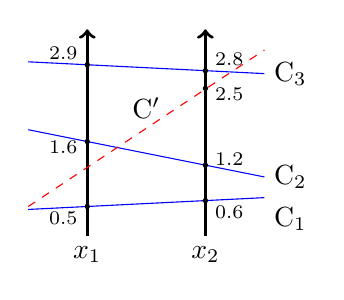
\begin{tikzpicture}[scale=0.75]
			% Draw the arrows
			\draw[very thick, ->] (0,0) node[below] {$x_1$} -- (0,3.5) ;
			\draw[very thick, ->] (2,0) node[below] {$x_2$} -- (2,3.5) ;
			
			% Draw the lines with labels extended further left and right
			\draw[blue] (-1,0.45) -- (3,0.65) node[right, below right, black] {C$_1$};
			\draw[blue] (-1,1.8) -- (3,1.0) node[right, black] {C$_2$};
			\draw[blue] (-1,2.95) -- (3,2.75) node[right, black] {C$_3$};
			
			% Dashed line extended further left and right
			\draw[red, dashed] (-1,0.5) -- (3,3.15) node[midway, above, black] {C$'$};
			
			% Labels on the left arrow with markers
			\node[left] at (0,0.3) {{\scriptsize 0.5}};
			\node[left] at (0,1.5) {{\scriptsize 1.6}};
			\node[left] at (0,3.1) {{\scriptsize 2.9}};
			\draw[fill=black] (0,0.5) circle (1pt);
			\draw[fill=black] (0,1.6) circle (1pt);
			\draw[fill=black] (0,2.9) circle (1pt);
			
			% Labels on the right arrow with markers
			\node[right] at (2,0.4) {{\scriptsize 0.6}};
			\node[right] at (2,1.3) {{\scriptsize 1.2}};
			\node[right] at (2,2.4) {{\scriptsize 2.5}};
			\node[right] at (2,3.0) {{\scriptsize 2.8}};	
			\draw[fill=black] (2,0.6) circle (1pt);
			\draw[fill=black] (2,1.2) circle (1pt);
			\draw[fill=black] (2,2.5) circle (1pt);
			\draw[fill=black] (2,2.8) circle (1pt);
		\end{tikzpicture}
		\caption{A distributed signal in with consistent cuts $C_1, C_2, C_3$ constituting a consistent cut flow. Note that $C'$ is a non-example since $(2.5, x_2(2.5)) \in \fr(C')$~and $(1.6, x_1(1.6)) \notin \fr(C')$,~but  $(1.6, x_1(1.6))$~happened
			before~$(2.5, x_2(2.5))$.} \label{fig:distsig}
		%	\vspace{1em}
	\end{figure}
	
	For all $T,T' \in \R_{\geq 0}$ and $1 \leq i \leq n$, if $T < T'$, then for every pair of events $(c_i(T), x_i(c_i(T))) \in \ccf(T)$ and $(c_i(T'), x_i(c_i(T'))) \in \ccf(T')$ we have $(c_i(T), x_i(c_i(T))) \hb (c_i(T'), x_i(c_i(T')))$.
	We denote by $\CCF(S,{\hb})$ the set of all consistent cut flows of the distributed signal $(S,{\hb})$.
	
	
	%\begin{example} \label{ex:distsig}
	%	Let $(S,{\hb})$ be a distributed signal with $S = (x_1, x_2)$ and $\varepsilon = 0.5$, where some events of $x_1$ and $x_2$ are marked on \cref{fig:distsig}.
	%	For example, $(0.5, x_1(0.5)) \hb (1.6, x_1(1.6)) \hb (2.5, x_2(2.5)) \hb (2.8, x_2(2.8))$, but $(2.5, x_2(2.5)) \not\hb (2.9, x_1(2.9))$.
	%	The solid blue lines marked with $C_1, C_2, C_3$ correspond to a consistent cut, e.g., $\fr(C_3) = \{(2.9, x_1(2.9)), (2.8, x_2(2.8))\}$, however $C'$ is not a consistent cut since $(2.5, x_2(2.5)) \in \fr(C')$ and $(1.6, x_1(1.6)) \hb (2.5, x_2(2.5))$ but $(1.6, x_1(1.6)) \notin \fr(C')$.
	%	Moreover, the frontiers of these consistent cuts can be seen as produced by a consistent cut flow $\ccf$, e.g., with $\ccf(0.5) = \fr(C_1)$, $\ccf(1) = \fr(C_2)$, and $\ccf(2) = \fr(C_3)$.	
	%\end{example}
	
	%\begin{wrapfigure}{r}{0.3\textwidth}
	%	\vspace{-2em}
	%	\begin{center}
		%		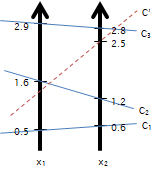
\includegraphics[scale=0.9]{distsig.png}
		%	\end{center}
	%	\caption{The distributed signal in \cref{ex:distsig} with consistent cuts $C_1, C_2, C_3$}
	%	\label{fig:distsig}
	%\end{wrapfigure}
	
	
	
	Observe that a consistent cut flow of a distributed signal induces a vector of synchronous signals which can be evaluated using the standard STL semantics described above.
	Let $(S,{\hb})$ be a distributed signal of $n$ signals $x_1, \ldots, x_n$.
	A consistent cut flow $\ccf \in \CCF(S,{\hb})$ yields a trace $w_{\ccf} = (x'_1, \ldots x'_n)$ on the temporal domain $[0,d)$ such that $(c_i(T), x_i(c_i(T))) \in \ccf(T)$ implies $x_i'(T) = x_i(c_i(T))$ for all $1 \leq i \leq n$ and $T \in [0, d)$.
	The set of traces of $(S,{\hb})$ is given by $\tr(S,{\hb}) = \{ w_{\ccf} \st \ccf \in \CCF(S,{\hb})\}$.
	
	We define the satisfaction of an STL formula $\varphi$ by a distributed signal $(S,{\hb})$ over a three-valued domain $\{\top, \bot, {?}\}$
	%If the set of synchronous traces $\tr(S,{\hb})$ defined by a distributed signal $(S,{\hb})$ is contained in the set of traces allowed by the formula $\varphi$, then $(S,{\hb})$ satisfies $\varphi$.
	%Similarly, if $\tr(S,{\hb})$ has an empty intersection with the set of traces $\varphi$ defines, then $(S,{\hb})$ violates $\varphi$.
	%Otherwise, the evaluation is inconclusive since some traces satisfy the property and some violate it.
	Notice that we quantify universally over traces for both satisfaction and violation.
	
	%\vspace{-1em}
	%\footnotesize
	\begin{equation*}
		[(S,{\hb}) \models \varphi] = 
		\begin{cases}
			\top \text{ if } \forall w \in \tr(S,{\hb}) : w \models \varphi \\
			\bot \text{ if } \forall w \in \tr(S,{\hb}) : w \models \lnot\varphi \\
			\,?\, \text{ otherwise}
		\end{cases}
	\end{equation*}
	%\normalsize
	
	
	
	\section{Overapproximation of the STL Distributed Semantics}
	\label{sec:semantics}
	
	To address the computational overhead in exact distributed monitoring, we define STL$^+$, a variant of STL whose syntax is the same as STL but semantics provide a sound approximation of the STL distributed semantics.
	In particular, given a distributed signal $(S,{\hb})$, STL$^+$ considers an approximation 
	$\tr^+(S,{\hb})$ of the set $\tr(S,{\hb})$ of synchronous traces where $ \tr(S,{\hb}) \subseteq \tr^+(S,{\hb})$.
	A signal $(S,{\hb})$ satisfies (resp. violates) an STL$^+$ formula $\varphi$ iff all the traces in $\tr^+(S,{\hb})$ belong to the language of $\varphi$ (resp. $\lnot \varphi$).
	
	%\vspace{-1em}
	%\footnotesize
	\begin{equation*}
		[(S,{\hb}) \models \varphi]_+ = 
		\begin{cases}
			\top \text{ if } \forall w \in \tr^+(S,{\hb}) : w \models \varphi \\
			\bot \text{ if } \forall w \in \tr^+(S,{\hb}) : w \models \lnot\varphi \\
			\,?\, \text{ otherwise}
		\end{cases}
	\end{equation*}
	%\normalsize
	
	%%% this may be not wlog -- the verdict may change when a formula is made copyless
	Throughout the paper, we assume  $\varphi$ is \emph{copyless}, i.e., each signal $x \in S$ occurs in $\varphi$ at most once.
	Moreover, the signals are Boolean, non-Zeno, piecewise-constant, and have no edge at time 0.
	We assume Boolean signals only for convenience; all the concepts and results generalize to non-Boolean signals because finite-length piecewise-constant signals use only a finite number of values.
	We note that our approach is a sound overapproximation also for non-copyless formulas, although potentially less precise.
	
	
	In \cref{sec:approach}, we define $\tr^+$ show that it overapproximates $\tr$ (\cref{cl:trsound}), which implies the soundness of STL$^+$ as stated in \cref{cl:stlsound}.
	In \cref{sec:algorithm} we present algorithm to compute the semantics of STL$^+$ and extend it to online monitoring.
	
	\begin{theorem} \label{cl:stlsound}
		Consider a distributed signal $(S,{\hb})$ and an STL formula $\varphi$.
		The following implications hold:
		\begin{align*}
			[(S,{\hb}) \models \varphi]_+ = \top &\implies [(S,{\hb}) \models \varphi] = \top \\
			[(S,{\hb}) \models \varphi]_+ = \bot &\implies [(S,{\hb}) \models \varphi] = \bot \\
		\end{align*}
	\end{theorem}
	\begin{proof}[\normalsize Proof.]
		\normalsize
		Let $\varphi$ be an STL formula and $(S,{\hb})$ be a distributed signal.
		Assume $[(S,{\hb}) \models \varphi]_+ = \top$.
		We want to show that $[(S,{\hb}) \models \varphi] = \top$.
		Expanding the definition of $[(S,{\hb}) \models \varphi]_+ = \top$, we have $w \models \varphi$ for all $w \in \tr^+(S,{\hb})$.
		By \cref{cl:trsound}, we have $\tr(S,{\hb}) \subseteq \tr^+(S,{\hb})$.
		Then, it holds that $w \models \varphi$ for all $w \in \tr(S,{\hb})$.
		Therefore, $[(S,{\hb}) \models \varphi] = \top$ by definition.
		The case of $[(S,{\hb}) \models \varphi]_+ = \bot$ follows from the same arguments.
	\end{proof}
	
	
	Notice that both the distributed semantics of STL and the semantics of STL$^+$ quantify universally over the set of traces for the verdicts $\top$ and $\bot$.
	Therefore, \cref{cl:stlsound} holds for the verdicts $\top$ and $\bot$, but not for ${\,?}$.
	
	
	\section{Overapproximation of Synchronous Traces} 
	\label{sec:approach}
	
	In this section, given a distributed signal $(S,{\hb})$, we describe an overapproximation $\tr^+(S,{\hb})$ of its set $\tr(S,{\hb})$ of synchronous traces.
	First, we present the notion of \emph{canonical segmentation}, a systematic way of partitioning the temporal domain of a distributed signal to track partial synchrony.
	Second, we introduce \emph{value expressions}, sets of finite words representing signal behavior in a time interval.
	Finally, we define $\tr^+$ and show that it soundly approximates $\tr$.
	
	%\begin{remark}
	%	We assume Boolean signals for convenience. 
	%	All the concepts and results in this section generalize to non-Boolean signals because finite-length piecewise-constant signals use only a finite number of values.
	%\end{remark}
	
	\paragraph*{Canonical Segmentation.}
	Consider a Boolean signal $x$ with a rising edge at time $t > \varepsilon$.
	Due to clock skew, this edge occurs in the range $(t - \varepsilon, t + \varepsilon)$ from the monitor's perspective.
	This range is an \emph{uncertainty region} because within it, the monitor can only tell that $x$ changes from 0 to 1. Formally, given an edge $(t, x(t))$, we define $\theta_{\text{lo}}(x,t) = \max(0, t - \varepsilon)$ and $\theta_{\text{hi}}(x,t) = \min(d, t + \varepsilon)$ as the endpoints of the edge's uncertainty region.
	
	Given a temporal domain $I = [0,d) \subset \R_{\geq 0}$, a \emph{segmentation} of $I$ is a partition of $I$ into finitely many intervals $I_1, \ldots, I_k$, called \emph{segments}, of the form $I_j = [t_j, t_{j+1})$ such that $t_j < t_{j+1}$ for all $1 \leq j \leq k$.
	By extension, a segmentation of a collection of signals with the same temporal domain $I$ is a segmentation of $I$.
	
	%Let $x : [0,d) \to \R$ be a signal and $(t, x(t))$ be an edge of $x$. %$E_x = \{(t_1, x(t_1)), \ldots, (t_m, x(t_m))\}$ be the set of edges of $x$, given in an increasing order of local clock values.
	%We define $\theta_{\text{lo}}(x,t) = \max(0, t - \varepsilon)$ and $\theta_{\text{hi}}(x,t) = t + \varepsilon$.
	%%\begin{align*}
	%%	%	\theta_{\text{lo}}(x,t_i) &= \max\{0, \max_{j \in \{1, i\}} t_j - \varepsilon - (j-i)\delta\} \text{, and} \\
	%%	\theta_{\text{lo}}(x,t_i) &= \max_{1 \leq j \leq i} t_j - \varepsilon + (i-j)\delta \text{, and} \\
	%%	\theta_{\text{hi}}(x,t_i) &= \min_{i \leq j \leq m} t_j + \varepsilon - (j-i)\delta.
	%%\end{align*}
	%Intuitively, $\theta_{\text{lo}}$ and $\theta_{\text{hi}}$ give us the lower and upper bounds on the value of the monitor's clock for a given edge, i.e., the end points of the uncertainty region of the given edge.
	%We use these to describe a canonical segmentation of a distributed signal.
	
	Let $(S,{\hb})$ be a distributed signal of $n$ signals.
	The \emph{canonical segmentation} $G_S$ of $(S,{\hb})$ the segmentation of $S$ where the segment endpoints match the temporal domain and uncertainty region endpoints.
	Formally, we define $G_S$ as follows.
	For each signal $x_i$, where $1 \leq i \leq n$, let $F_i$ be the set of uncertainty region endpoints.
	Let $F = \{0, d\} \cup \bigcup_{i = 1}^{n} F_i$ and let $(s_j)_{1 \leq j \leq |F|}$ be a nondecreasing sequence of clock values corresponding to the elements of $F$.
	Then, the canonical segmentation of $(S,{\hb})$ is $G_S = \{I_1, \ldots, I_{|F| - 1}\}$ where $I_j = [s_j, s_{j+1})$ for all $1 \leq j < |F|$.
	We show an example in \cref{fig:csve}a.
	
	%\begin{example} \label{ex:canonseg}
	%	\ege{remove?}
	%	Let $(S, {\hb})$ be a distributed Boolean signal with $S = (x_1, x_2)$ and $\varepsilon = 2$ over the temporal domain $[0,8)$.
	%	Both signals are initially 0.
	%	Signal $x_1$ has a rising edge at time 2 and a falling edge at time 5, while $x_2$ has a rising edge at time 3 and a falling edge at time 6.
	%	The uncertainty regions of $x_1$ are $(0,4)$ and $(3,7)$, while those of $x_2$ are $(1,5)$ and $(4,8)$.
	%	Then, we have $F = \{0, 8\} \cup \{0, 1, 3, 4, 5, 7, 8\}$, and thus the canonical segmentation is $G_S = \{ [0,1), [1,3), [3,4), [4,5), [5,7), [7,8) \}$.
	%\end{example}
	
	\begin{figure*}
		%	\vspace{-1em}
		\centering
		\begin{subfigure}[c]{.45\textwidth}
			\centering
			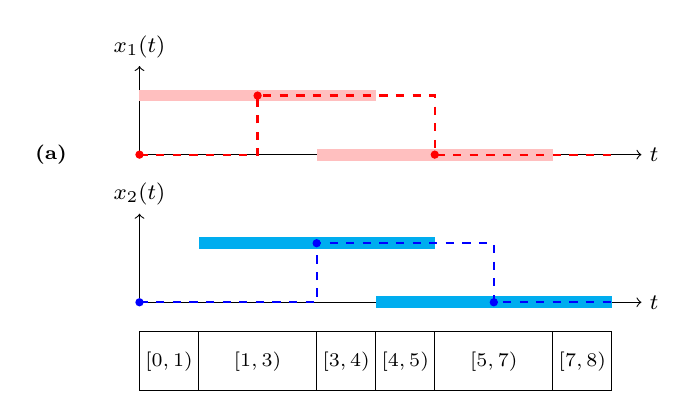
\begin{tikzpicture}[scale=0.75]
				\scriptsize
				\node at (-1.5,0) {\textbf{(a)}};
				\footnotesize 
				% Plot for x1(t)
				\begin{scope}
					% Axes
					\draw[->] (0,0) -- (8.5,0) node[right] {$t$};
					\draw[->] (0,0) -- (0,1.5) node[above] {$x_1(t)$};
					
					% Red shaded areas
					\fill[pink] (0,1.1) rectangle (4,0.9);
					\fill[pink] (3,0.1) rectangle (7,-0.1);
					
					% Red dashed lines
					\draw[red, thick, dashed] (0,0) -- (2,0) -- (2,1) -- (5,1) -- (5,0) -- (8,0);
					
					% Red dots
					\fill[red] (0,0) circle (2pt);
					\fill[red] (2,1) circle (2pt);
					\fill[red] (5,0) circle (2pt);
				\end{scope}
				
				% Plot for x2(t)
				\begin{scope}[shift={(0,-2.5)}]
					% Axes
					\draw[->] (0,0) -- (8.5,0) node[right] {$t$};
					\draw[->] (0,0) -- (0,1.5) node[above] {$x_2(t)$};
					
					% Red shaded areas
					\fill[cyan] (1,1.1) rectangle (5,0.9);
					\fill[cyan] (4,0.1) rectangle (8,-0.1);
					
					% Red dashed lines
					\draw[blue, thick, dashed] (0,0) -- (3,0) -- (3,1) -- (6,1) -- (6,0) -- (8,0);
					
					% Red dots
					\fill[blue] (0,0) circle (2pt);
					\fill[blue] (3,1) circle (2pt);
					\fill[blue] (6,0) circle (2pt);
				\end{scope}
				
				% GS boxes
				\begin{scope}[shift={(0,-4)}]
					\draw (0,0) rectangle (1,1);
					\node at (0.5,0.5) {{\scriptsize $[0,1)$}};
					\draw (1,0) rectangle (3,1);
					\node at (2,0.5) {{\scriptsize $[1,3)$}};
					\draw (3,0) rectangle (4,1);
					\node at (3.5,0.5) {{\scriptsize $[3,4)$}};
					\draw (4,0) rectangle (5,1);
					\node at (4.5,0.5) {{\scriptsize $[4,5)$}};
					\draw (5,0) rectangle (7,1);
					\node at (6,0.5) {{\scriptsize $[5,7)$}};
					\draw (7,0) rectangle (8,1);
					\node at (7.5,0.5) {{\scriptsize $[7,8)$}};
				\end{scope}
			\end{tikzpicture}
		\end{subfigure}
		\hspace{2em}
		\begin{subfigure}[c]{.45\textwidth}
			\centering
			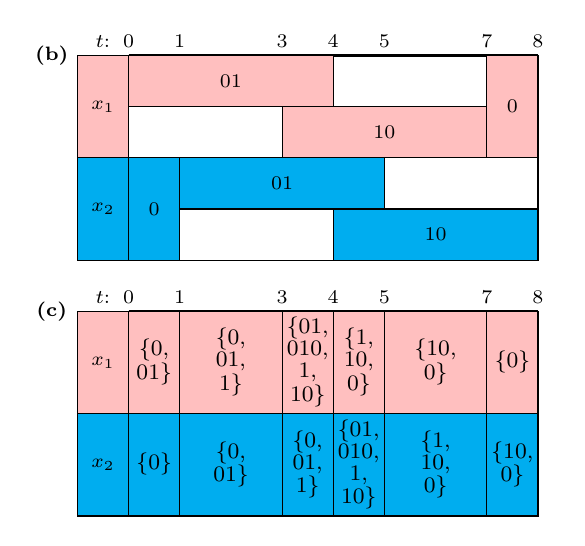
\begin{tikzpicture}[scale=0.65]
				\scriptsize
				% Part (a)
				\node at (-1.5,0) {\textbf{(b)}};
				\draw[thick] (0,0) -- (8,0);
				\foreach \x in {0,1,3,4,5,7,8}
				\draw (\x,0) node[above] {\x};
				\draw (-0.5,0) node[above] {$t$:};
				
				\draw[fill=pink] (-1,-2) rectangle (0,0) node[midway] {$x_1$};
				\draw[fill=pink] (0,-1) rectangle (4,0) node[midway] {$01$};
				\draw[fill=pink] (3,-2) rectangle (7,-1) node[midway] {$10$};
				\draw[fill=pink] (7,-2) rectangle (8,0) node[midway] {$0$};
				
				\draw[fill=cyan] (-1,-4) rectangle (0,-2) node[midway] {$x_2$};
				\draw[fill=cyan] (0,-4) rectangle (1,-2) node[midway] {$0$};
				\draw[fill=cyan] (1,-3) rectangle (5,-2) node[midway] {$01$};
				\draw[fill=cyan] (4,-4) rectangle (8,-3) node[midway] {$10$};
				
				\draw (0,-4) -- (8,-4);
				\draw (8,-4) -- (8,0);
				
				% Part (b)
				\node at (-1.5,-5) {\textbf{(c)}};
				\draw[thick] (0,-5) -- (8,-5);
				\foreach \x in {0,1,3,4,5,7,8}
				\draw (\x,-5) node[above] {\x};
				\draw (-0.5,-5) node[above] {$t$:};
				
				\draw[fill=pink] (-1,-7) rectangle (0,-5) node[midway] {$x_1$};
				\draw[fill=pink] (0,-7) rectangle (1,-5) node[midway] { \fontsize{8}{8}\selectfont \begin{tabular}{c}\{0,\\ 01\}\\\end{tabular}};
				\draw[fill=pink] (1,-7) rectangle (3,-5) node[midway] {\fontsize{8}{8}\selectfont\begin{tabular}{c}\{0,\\ 01,\\ 1\}\\\end{tabular}};
				\draw[fill=pink] (3,-7) rectangle (4,-5) node[midway] {\fontsize{8}{8}\selectfont{\begin{tabular}{c}\{01,\\ 010,\\ 1,\\ 10\}\\\end{tabular}}};
				\draw[fill=pink] (4,-7) rectangle (5,-5) node[midway] {\fontsize{8}{8}\selectfont\begin{tabular}{c}\{1,\\ 10,\\ 0\}\\\end{tabular}};
				\draw[fill=pink] (5,-7) rectangle (7,-5) node[midway] {{\fontsize{8}{8}\selectfont\begin{tabular}{c}\{10,\\ 0\}\\\end{tabular}}};
				\draw[fill=pink] (7,-7) rectangle (8,-5) node[midway] {{\fontsize{8}{8}\selectfont\begin{tabular}{c}\{0\}\\\end{tabular}}};
				
				\draw[fill=cyan] (-1,-9) rectangle (0,-7) node[midway] {$x_2$};
				\draw[fill=cyan] (0,-9) rectangle (1,-7) node[midway] {{\fontsize{8}{8}\selectfont\begin{tabular}{c}\{0\}\\\end{tabular}}};
				\draw[fill=cyan] (1,-9) rectangle (3,-7) node[midway] {\fontsize{8}{8}\selectfont\begin{tabular}{c}\{0,\\ 01\}\\\end{tabular}};
				\draw[fill=cyan] (3,-9) rectangle (4,-7) node[midway] {\fontsize{8}{8}\selectfont\begin{tabular}{c}\{0,\\ 01,\\ 1\}\\\end{tabular}};
				\draw[fill=cyan] (4,-9) rectangle (5,-7) node[midway] {\fontsize{8}{8}\selectfont{\begin{tabular}{c}\{01,\\ 010,\\ 1,\\ 10\}\\\end{tabular}}};
				\draw[fill=cyan] (5,-9) rectangle (7,-7) node[midway] {\fontsize{8}{8}\selectfont\begin{tabular}{c}\{1,\\ 10,\\ 0\}\\\end{tabular}};
				\draw[fill=cyan] (7,-9) rectangle (8,-7) node[midway] {{\fontsize{8}{8}\selectfont\begin{tabular}{c}\{10,\\ 0\}\\\end{tabular}}};
			\end{tikzpicture}
		\end{subfigure}
		\vspace{1ex}	
		\caption{\textbf{(a)} A distributed signal $(S,{\hb})$ with $x_1$ (top, red) and $x_2$ (bottom, blue) whose edges are marked with solid balls and their uncertainty regions are given as semi-transparent boxes around the edges. The resulting canonical segmentation $G_S$ is shown below the graphical representation of the signals. \textbf{(b)} The uncertainty regions of $(S,{\hb})$ and the corresponding value expressions. \textbf{(c)} The tabular representation of the function $\gamma$ for $(S,{\hb})$, e.g., \(\gamma(x_1, [3,4)) = (\sfx(01) \cdot \pfx(10)) \setminus \{\epsilon\} = \{ 01, 010, 1, 10\}\).\label{fig:csve}}
		%	\vspace{1em}
	\end{figure*}
	
	
	\paragraph*{Value Expressions.}
	Consider a Boolean signal \( x \) with a rising edge within an uncertainty region of \((t_1, t_2)\).
	As mentioned, the monitor only knows that \( x \) changes from 0 to 1 in this interval.
	This knowledge is represented as a finite word \( v = 01 \) over the alphabet \(\Sigma = \{0,1\}\).
	This representation, called a \emph{value expression}, encodes the uncertain behavior of an observed signal relative to the monitor.
	Formally, a value expression is an element of \(\Sigma^*\), where \(\Sigma\) is the finite alphabet of signal values.
	Given a signal \( x \) and an edge \((t, x(t))\), the value expression corresponding to the uncertainty region \((\theta_{\text{lo}}(x,t), \theta_{\text{hi}}(x,t))\) is \( v_{x,t} = v_- \cdot v_+ \), where \( v_- = \lim_{s \to t^-} x(s) \) and \( v_+ = \lim_{s \to t^+} x(s) \).
	We omit the concatenation symbol \(\cdot\) when the letters are clear from context.
	This definition is general because finite-length piecewise-constant real-valued signals will only have a finite number of values, making \(\Sigma\) finite.
	
	Notice that (i) uncertainty regions may overlap, and (ii) the canonical segmentation may split an uncertainty region into multiple segments.
	Consider a signal $x$ with a rising edge in $(1,5)$ and a falling edge in $(4,8)$.
	The corresponding value expressions are respectively $v_1 = 01$ and $v_2 = 10$.
	Notice that the behavior of $x$ in the interval $[1,4)$ can be expressed as $\pfx(v_1)$, encoding whether the rising edge has happened yet.
	Similarly, the behavior in $[4,5)$ is given by $\sfx(v_1) \cdot \pfx(v_2)$, which captures whether the edges occur in this interval (thanks to prefixing and suffixing) and the fact that the rising edge happens before the falling edge (thanks to concatenation).
	
	%\begin{wrapfigure}{r}{0.5\textwidth}
	%	%	\vspace{-2em}
	%	
	%
	%\end{wrapfigure}
	
	Formally, given a distributed signal $(S,{\hb})$, we define a function $\gamma : S \times G_S \to 2^{\Sigma^*}$ that maps each signal and segment of the canonical segmentation to a set of value expressions, capturing the signal's potential behaviors in the given segment.
	Let $x$ be a signal in $S$, and let $R_1, \ldots, R_m$ be its uncertainty regions where $R_i = (t_i, t_i')$ and the corresponding value expression is $v_i$ for all $1 \leq i \leq m$.
	Now, let $I \in G_S$ be a segment with $I = [s, s')$ and for each $1 \leq i \leq m$ define the set $V_i$ of value expressions capturing how $I$ relates with $R_i$ in \cref{eq:valexprset}.
	%
	\begin{figure}
		%	\small
		%	\vspace{-1em}
		\begin{equation} \label{eq:valexprset}
			V_i = 
			\begin{cases}
				\{v_i\} & \text{if } t_i = s \land s' = t_i' \\
				\pfx(v_i) & \text{if } t_i = s \land s' < t_i' \\
				\sfx(v_i) & \text{if } t_i > s \land s' = t_i' \\
				\infx(v_i) & \text{if } t_i > s \land s' < t_i' \\
				\{\epsilon\} & \text{otherwise}
			\end{cases}
		\end{equation}
		%	\vspace{-2em}
	\end{figure}
	%\normalsize
	The last case happens only when \( I \cap R_i \) is empty.
	We define \(\gamma\) as follows:
	%%\vspace{-1em}
	\[ \gamma(x,I) = \destutter(V_1 \cdot V_2 \cdot \ldots \cdot V_m) \setminus \{\epsilon\} \]
	%%\vspace{-1em}
	Observe that \(\gamma(x,I)\) contains all the potential behaviors of \( x \) in segment \( I \) by construction.
	However, it is potentially overapproximate because the sets \( V_1, \ldots, V_m \) contain redundancy by definition, and the concatenation does not ensure that an edge is considered exactly once -- see \cref{fig:csve}b and \cref{fig:csve}c.
	%We demonstrate this in \cref{fig:csve}b and \cref{fig:csve}c.
	
	%\begin{example} \label{ex:valexpr}
	%	Recall the distributed signal \((S, {\hb})\) in \cref{fig:canonseg}.
	%	In \cref{fig:valexpr}a, we show the value expressions corresponding to its uncertainty regions.
	%	For example, the falling edge of \(x_1\) has an uncertainty region of \((3,7)\), represented by the value expression \(10\). 
	%	In \cref{fig:valexpr}b, we give the function \(\gamma\) for \((S, {\hb})\).
	%	For example, \(\gamma(x_1, [3,4)) = (\sfx(01) \cdot \pfx(10)) \setminus \{\epsilon\} = \{ 01, 010, 1, 10\}\), and \(\gamma(x_2, [0,1)) = \{0\}\).
	%\end{example}
	
	
	
	
	\paragraph*{Overapproximation of $\tr$.}
	Consider a distributed signal $(S,{\hb})$ of $n$ signals, and let $G_S$ be its canonical segmentation.
	We describe how the function $\gamma$ defines a set $\tr^+(S,{\hb})$ of synchronous traces that overapproximates the set $\tr(S,{\hb})$.
	%
	%Let $x : [0,d) \to \B$ be a signal.
	%Consider the set $N_x$ of signals such that each $x' \in X$ is obtained from $x$ by shifting its edges within their uncertainty regions while preserving their relative order.
	%Formally, we let $E = \{ (t_1, x(t_1)), \ldots, (t_m, x(t_m)) \}$ be the set of edges of $x$ with $t_i < t_{i+1}$ for all $1 \leq i < m$, let $R_1, \ldots, R_m$ be the corresponding uncertainty regions, and define $N_x$ as follows: 
	%$$ N_x = \{x' : [0,d) \to \B \st x'(0) = x(0) \land \forall 1 \leq i \leq m : t_i' \in R_i \land x'(t_i') = x(t_i) \} $$ where $E' = \{ (t_1', x'(t_1')), \ldots, (t_m', x'(t_m')) \}$ is the set of edges of $x'$ with $t_i' < t_{i+1}'$ for all $1 \leq i < m$.
	%For example, ...
	%
	%Now, 
	%Let $x \in S$ and $x'$ be two signals with the same temporal domain, and let $I = [s, s')$ be a segment in $G_S$.
	%Let $(t_1, x'(t_1)), \ldots, (t_\ell, x'(t_\ell))$ be the edges of $x'$ in segment $I$ with $t_i < t_{i+1}$ for all $1 \leq i < \ell$.
	%The signals $x$ and $x'$ are \emph{consistent in $I$} iff $x(s) = x'(s)$ and the value expression $x'(s) \cdot x'(t_1) \cdot \ldots \cdot x'(t_\ell)$ belongs to $\gamma(x,I)$.
	%Moreover, $x$ and $x'$ are \emph{consistent} iff they are consistent in $I$ for all $I \in G_S$.
	%Now, let $S = (x_1, \ldots, x_n)$ and define the \emph{canonical overapproximation} of $(S,{\hb})$ as follows:
	%$$ \tr^+(S,{\hb}) = \{ (x_1', \ldots, x_n') \st \text{$x_i$ and $x_i'$ are consistent for all $1 \leq i \leq n$}\} $$
	%
	Consider $x \in S$, and let $x'$ be a signal with the same temporal domain, and let $I = [s, s')$ be a segment in $G_S$.
	Let $(t_1, x'(t_1)), \ldots, (t_\ell, x'(t_\ell))$ be the edges of $x'$ in segment $I$ with $t_i < t_{i+1}$ for all $1 \leq i < \ell$.
	The signal $x'$ is \emph{$I$-consistent with $x$} iff the value expression $x'(s) \cdot x'(t_1) \cdot \ldots \cdot x'(t_\ell)$ belongs to $\gamma(x,I)$.
	Moreover, $x'$ is \emph{consistent with $x$} iff it is $I$-consistent with $x$ for all $I \in G_S$.
	Now, let $S = (x_1, \ldots, x_n)$ and define $\tr^+(S,{\hb})$ as follows:
	%\vspace{-0.5em}
	\begin{align*}
		\tr^+(S,{\hb}) = \{ (x_1', \ldots, x_n') \st \text{$x_i'$ is consistent with}&\\
		\text{$x_i$ for all $1 \leq i \leq n$}&\} 
	\end{align*}
	%%\vspace{-1em}
	
	
	\begin{example} \label{ex:overapx}
		Recall \((S, {\hb})\) and its \(\gamma\) function from \cref{fig:csve}.
		Consider the synchronous trace \(w \in \tr(S, {\hb})\) where the rising edges of both signals occur at time 3 and the falling edges at time 5.
		Such a signal \( w \) would be included in \(\tr^+(S,{\hb})\) since for each \(i \in \{1,2\}\), the value expression 1 is contained in \(\gamma(x_i, [3,4))\) and \(\gamma(x_i, [4,5))\), while 0 is contained in the remaining sets \(\gamma\) maps \(x_i\) to.
		Now, consider a synchronous trace \((x_1', x_2')\) where both signals are initially 0, have rising edges at time 2 and 3.5, and falling edges at time 3 and 5.
		This trace does not belong to \(\tr(S, {\hb})\) since \(x_1'\) and \(x_2'\) have more edges than \(x_1\) and \(x_2\).
		However, it belongs to \(\tr^+(S,{\hb})\) since \(x_1'\) and \(x_2'\) are consistent with \(x_1\) and \(x_2\).
		Specifically, for each \(i \in \{1,2\}\), the value expression \(01\) is contained in \(\gamma(x_i, [1,3))\) and \(\gamma(x_i, [3,4))\), the expression \(1\) is contained in \(\gamma(x_i, [4,5))\), and 0 is contained in the remaining sets \(\gamma\) maps \(x_i\) to.
	\end{example}
	
	Notice that any trace in $\tr(S,\hb)$ can be seen as an $\varepsilon$-retiming of the original signal.
	Putting it all together, we finally prove that $\tr^+$ overapproximates $\tr$.
	
	\begin{lemma} \label{cl:trsound}
		For every distributed signal $(S,{\hb})$, we have $\tr(S,{\hb}) \subseteq \tr^+(S,{\hb})$.
	\end{lemma}
	\begin{proof}[\normalsize Proof.]
		\normalsize
		Let $(S,{\hb})$ be a distributed signal where $S = (x_1, \ldots, x_n)$.
		Let $w = (y_1, \ldots, y_n) \in \tr(S,{\hb})$ be a trace.
		We want to show that $w \in \tr^+(S,{\hb})$.
		First, let us recall the definition of $\tr^+$.
		\begin{align*}
			\tr^+(S,{\hb}) = \{ (x_1', \ldots, x_n') \st \text{$x_i'$ is consistent with}&\\
			\text{$x_i$ for all $1 \leq i \leq n$}&\} 
		\end{align*}
		
		Let $1 \leq i \leq n$ be arbitrary.
		To show that $y_i$ is consistent with $x_i$, we need to show that $y_i$ is $I$-consistent with $x_i$ for all $I \in G_S$.
		Let $I = [t_0, s)$ be an arbitrary segment in $G_S$, let $(t_1, y_i(t_1)), \ldots, (t_\ell, y_i(t_\ell))$ be the edges of $y_i$ in segment $I$ with $t_j < t_{j+1}$ for all $1 \leq j < \ell$.
		To show that $y_i$ is $I$-consistent with $x_i$, we need to show that the expression $y_i(t_0) \cdot y_i(t_1) \cdot \ldots \cdot y_i(t_\ell)$ belongs to $\gamma(x_i,I)$.
		We sketch the proof idea below.
		
		Note that $w$ can be seen as a trace obtained through an $\varepsilon$-retiming of $S$ (\cite[Section 4.2]{MomtazAB23}).
		Then, the timestamp $t$ of any edge of $x_i$ is mapped to some clock value in the range $(\theta_{\text{lo}}(t), \theta_{\text{hi}}(t))$.
		In particular, $|t - c^{-1}_i(t)| < \varepsilon$ for all $t \in \{t_0, t_1, \ldots, t_\ell\}$, where $c^{-1}_i(t)$ is the local clock value of $x_i$ mapped to $t$.
		
		Since $y_i$ has $\ell$ edges in $I$, it holds that $x_i$ has at least $\ell$ edges in $(t_0 - \varepsilon, s + \varepsilon)$.
		Since $I$ is a segment in $G_S$, there are $\ell$ of these that are consecutive such that the intersection of their uncertainty regions contain $(t_0,s)$, i.e., $(t_0,s) \subseteq \bigcap_{1 \leq j \leq \ell} (\theta_{\text{lo}}(t_j'), \theta_{\text{hi}}(t_j'))$ where $t_j' = c^{-1}_i(t_j)$ is the corresponding timestamp in $x_i$ for all $0 \leq j \leq \ell$.
		In particular, note that $y_i(t_j) = x_i(t_j')$ for all $0 \leq j \leq \ell$.
		
		Now, notice that, by definition, $\gamma(x_i, I)$ takes into account every edge of $x_i$ whose uncertainty region has a nonempty intersection with $I$, and preserves their order.
		Let $V_j$ be the set of value expressions capturing how $I$ relates with the uncertainty intervals of the edge $(t_j', x_i(t_j'))$ for all $1 \leq j \leq \ell$ (as defined in \cref{eq:valexprset}).
		Then, $\destutter(\{x_i(t_0')\} \cdot V_1 \cdot \ldots \cdot V_\ell) \subseteq \gamma(x_i, I)$.
		One can verify that for all $1 \leq j \leq \ell$, either $x_i(t_j')$ or $x_i(t_{j-1}') \cdot x_i(t_j')$ belongs to $V_j$.
		This allows us to choose a value expression $v_j$ from each $V_j$ such that $\destutter(\{x_i(t_0')\} \cdot v_1 \cdot \ldots \cdot v_\ell) = x_i(t_0') \cdot x_i(t_1') \cdot \ldots \cdot x_i(t_\ell')$, which concludes the proof. 
		
		Note that if there are more edges of $x_i$ with a timestamp smaller than $t_0'$ or larger than $t_\ell'$ whose uncertainty intervals intersect with $I$, then the corresponding set of value expressions is obtained either by prefixing or suffixing.
		In either case, we can choose $\epsilon$ from these sets for concatenation with the remaining edges' value expressions and obtain the desired result.
	\end{proof}
	
	\section{Monitoring Algorithm} 
	\label{sec:algorithm}
	
	\bgroup \color{red}
	In this section, we give algorithms to compute the STL$^+$ semantics in two different settings: the \emph{offline} setting where the entire execution trace is available at once (\cref{sec:offline}) and the \emph{online} setting where the execution trace becomes available incrementally (\cref{sec:online}).
	In the offline setting, our algorithm works both for future STL and past STL.
	In the online setting, we consider only past STL.
	\egroup
	
	\subsection{Offline Algorithm} \label{sec:offline}
	In the offline setting, we assume the entire signal is available to the monitor.
	We describe an algorithm, given a distributed signal $(S,{\hb})$ and an STL formula $\varphi$, to compute $[(S,{\hb}) \models \varphi]_+$ using the function $\gamma$ from \cref{sec:approach} without explicitly computing $\tr^+(S,{\hb})$.
	We introduce the \emph{asynchronous product} of value expressions to capture interleavings within segments, then evaluate \emph{untimed} and \emph{timed operators}.
	Finally, we combine these steps to compute the \emph{semantics} of STL$^+$.
	
	We also discuss an efficient implementation of the monitoring algorithm using \emph{bit vectors}, heuristics to enhance \emph{generalization} for real-valued signals, and a method to \emph{combine} our approach with exact monitoring.
	
	\paragraph*{Asynchronous Products.}
	Consider the value expressions $u_1 = 0 \cdot 1$ and $u_2 = 1 \cdot 0$ encoding the behaviors of two signals within a segment.
	Since behaviors within a segment are asynchronous, to capture their potential interleavings, we consider how the values in $u_1$ and $u_2$ can align.
	In particular, there are three potential alignments:
	(i) the rising edge of $u_1$ happens before the falling edge of $u_2$,
	(ii) the falling edge of $u_2$ happens before the rising edge of $u_1$, and
	(iii) they happen simultaneously.
	We respectively represent these with the tuples $(011, 110)$, $(001, 100)$, and $(01, 10)$ where the first component encodes $u_1$ and the second $u_2$.
	Formally, given two value expressions $u_1$ and $u_2$ (resp.  sets $L_1$ and $L_2$ of value expressions), we define their \emph{asynchronous product} as follows:
	
	\begin{align*}
		u_1 \otimes u_2 &=
		\begin{aligned}[t]
			\big\{ \destutter(v_1, v_2) \st v_i \in \stutter_k(u_i), \\
			k = |u_1| + |u_2| - 1, i \in \{1,2\} \big\}
		\end{aligned}\\
		L_1 \otimes L_2 &= \{ u_1 \otimes u_2 \st u_1 \in L_1, u_2 \in L_2 \}
	\end{align*}
	
	Asynchronous products of value expressions allow us to lift value expressions to satisfaction signals of formulas.
	
	\begin{example} \label{ex:asyncprod}
		Recall $(S, {\hb})$ and its $\gamma$ function given in \cref{fig:csve}.
		To compute the value expressions encoding the satisfaction of $x_1 \land x_2$ in the segment $[1,3)$, we first compute the asynchronous product $\gamma(x_1, [3,4)) \otimes \gamma(x_2, [3,4))$, and then the bitwise conjunction of each pair in the set.
		For example, taking the expression $0  1  0$ for $x_1$ and $0  1$ for $x_2$, the product contains the pair $(010, 011)$.
		Its bitwise conjunction is $0  1  0$, encoding a potential behavior for the satisfaction of $x_1 \land x_2$.
	\end{example}
	
	\paragraph*{Untimed Operations.}
	As hinted in \cref{ex:asyncprod}, to compute the semantics, we apply bitwise operations on value expressions and their asynchronous products to transform them into encodings of satisfaction signals of formulas.
	For example, to determine $[(S, {\hb}) \models \LTLeventually (x_1 \land x_2)]_+$, we first compute for each segment in $G_S$ the set of value expressions for the satisfaction of $x_1 \land x_2$, and then from these compute those of $\LTLeventually (x_1 \land x_2)$.
	This compositional approach allows us to evaluate arbitrary STL$^+$ formulas.
	
	\bgroup \color{red}
	First, we define bitwise operations on Boolean value expressions encoding atomic propositions.
	Then, we use these to evaluate untimed STL formulas over sets of value expressions.
	Let $u$ and $v$ be Boolean value expressions of length $\ell$.
	We denote by $u \BitAnd v$ the bitwise-and operation, by $u \BitOr v$ the bitwise-or, and by $\BitNeg u$ the bitwise-negation.
	We also define the \emph{bitwise strong until} and \emph{bitwise strong since} operators:
	\begin{align*}
		u \mathsf{U}^0 v &= \left( \max_{i \leq j \leq \ell} \left( \min \left( v[j], \min_{i \leq k \leq j} u[k] \right) \right) \right)_{1 \leq i \leq \ell} \\
		u \mathsf{S}^0 v &= \left( \max_{1 \leq j \leq i} \left( \min \left( v[j], \min_{j \leq k \leq i} u[k] \right) \right) \right)_{1 \leq i \leq \ell}
	\end{align*}
	As usual, we derive \emph{bitwise eventually} as 
	$\mathsf{E} u = 1^\ell \mathsf{U}^0 u$, \emph{bitwise always} as $\mathsf{A} u = \BitNeg 
	(\mathsf{E} \BitNeg u)$, and \emph{bitwise weak until} as $u \mathsf{U}^1 v = (u \mathsf{U}^0 v) 
	\BitOr (\mathsf{A} u)$.
	The corresponding past-time operations are defined similarly:
	$\bar{\mathsf{E}} u = 1^\ell \mathsf{S}^0 u$,
	$\bar{\mathsf{A}} u = \BitNeg (\bar{\mathsf{E}} \BitNeg u)$, and 
	$u \mathsf{S}^1 v = (u \mathsf{S}^0 v) \BitOr (\bar{\mathsf{A}} u)$.
	The distinction between $\mathsf{U}^0$ and $\mathsf{U}^1$ (resp. $\mathsf{S}^0$ and $\mathsf{S}^1$) will be useful when we incrementally evaluate a formula.
	Finally, note that the output of these operations is a value expression of length $\ell$.
	For example, if $u = 010$, we have $\mathsf{E} u = 110$ and $\mathsf{A} u = 000$.
	\egroup
	
	Let  $(S, {\hb})$ be a distributed signal.
	Consider an atomic proposition $p \in \AP$ encoded as $x_p \in S$ and let $\varphi_1, \varphi_2$ be two STL formulas.
	We define the evaluation of untimed formulas with respect to $(S, {\hb})$ and a segment $I \in G_S$ inductively as shown in \cref{fig:eval}.
	When $\varphi$ is a future (resp. past) formula and $I$ is the first (resp. last) segment in $G_S$, we simply write $\llbracket (S, {\hb}) \models \varphi \rrbracket$.
	
	\begin{figure*}[!t]
		\begin{align*}
			\llbracket (S, {\hb}), I \models p \rrbracket &= \gamma(x_p, I) \\
			\llbracket (S, {\hb}), I \models \lnot \varphi_1 \rrbracket &= \{\BitNeg u \st u \in  \llbracket (S, {\hb}), I \models \varphi_1 \rrbracket \} \\
			\llbracket (S, {\hb}), I \models \varphi_1 \land \varphi_2 \rrbracket &= \destutter(\{ u_1 \BitAnd u_2 \st (u_1, u_2) \in \llbracket (S, {\hb}), I \models \varphi_1 \rrbracket \otimes \llbracket (S, {\hb}), I \models \varphi_2 \rrbracket  \}) \\
			\llbracket (S, {\hb}), I \models \varphi_1 \until \varphi_2 \rrbracket &= \destutter(\{ u_1 \mathsf{U}^a u_2 \st (u_1, u_2) \in \llbracket (S, {\hb}), I \models \varphi_1 \rrbracket \otimes \llbracket (S, {\hb}), I \models \varphi_2 \rrbracket, \\
			&\hspace{17em} a \in \first(\llbracket (S, {\hb}), I' \models \varphi_1 \until \varphi_2 \rrbracket) \}) \\
			\bgroup \color{red}\llbracket (S, {\hb}), I \models \varphi_1 \since \varphi_2 \rrbracket \egroup &= \destutter(\{ u_1 \mathsf{S}^a u_2 \st (u_1, u_2) \in \llbracket (S, {\hb}), I \models \varphi_1 \rrbracket \otimes \llbracket (S, {\hb}), I \models \varphi_2 \rrbracket, \\
			&\hspace{17em} a \in \last(\llbracket (S, {\hb}), I'' \models \varphi_1 \since \varphi_2 \rrbracket) \})
		\end{align*}
		\caption{Inductive evaluation of untimed formulas, where $I'$ is the segment that follows $I$ in $G_S$  and  $I''$ is the segment that precedes $I$ in $G_S$ (if such segments exist). For completeness, for every formula $\varphi$ we define $\llbracket (S, {\hb}), J \models \varphi \rrbracket = \{0\}$ when $J \notin G_S$. \label{fig:eval}}
	\end{figure*}
	
	Similarly as above, we can use the standard derived operators to compute the corresponding sets of value expressions.
	For a given formula and a segment, the evaluation above produces a set of value expressions encoding the formula's satisfaction within the segment.
	
	\begin{example}
		Recall $(S, {\hb})$ and $\gamma$ from \cref{fig:csve}.
		To compute $\llbracket (S, {\hb}), [5,7) \models \LTLeventually(x_1 \land x_2) \rrbracket$, we first compute $\llbracket (S, {\hb}), [5,7) \models x_1 \land x_2 \rrbracket$ by taking the bitwise conjunction over the asynchronous product $\gamma(x_1, [5,7)) \otimes \gamma(x_2, [5,7))$ and destuttering.
		For example, since $010 \in \gamma(x_1, [5,7))$ and $01 \in \gamma(x_2, [5,7))$, the pair $(0010,0111)$ is in the product, whose conjunction gives us $010$ after destuttering. 
		Repeating this for the rest, we obtain $\llbracket (S, {\hb}), [5,7) \models x_1 \land x_2 \rrbracket = \{ 0, 01, 010, 1, 10 \}$.
		Finally, we compute $\llbracket (S, {\hb}), [5,7) \models \LTLeventually(x_1 \land x_2) \rrbracket$ by applying each expression in $\llbracket (S, {\hb}), [5,7) \models x_1 \land x_2 \rrbracket$ the bitwise eventually operator and destuttering.
		The resulting set $\{0, 1, 10\}$ encodes the satisfaction signal of $\LTLeventually(x_1 \land x_2)$ in $[5,7)$.
		Note that we do not need to consider the evaluation of the next segment for the eventually operator since $\llbracket (S, {\hb}), [7,8) \models x_1 \land x_2 \rrbracket = \{0\}$.
	\end{example}
	
	\paragraph*{Timed Operations.}
	Handling timed operations requires a closer inspection as value expressions are untimed by definition.
	We address this issue by considering how a given evaluation interval relates with a given segmentation.
	For example, take a segmentation $G_S = \{ [0,4), [4,6), [6,10) \}$ and an evaluation interval $J = [0,5)$.
	Suppose we are interested in how a signal $x \in S$ behaves with respect to $J$ over the first segment $I = [0,4)$.
	First, to see how $J$ relates with $G_S$ with respect to $I =[0,4)$, we  ``slide'' the interval $J$ over $I \oplus J = [0,9)$ and consider the different ways it intersects the segments in $G_S$.
	Initially, $J$ covers the entire segment $[0,4)$ and the beginning of $[4,6)$, for which the potential behaviors of $x$ are captured by the set $\gamma(x, [0,4)) \cdot \pfx(\gamma(x, [4,6)))$.
	Now, if we slide the window and take $J' = [3,7)$, the window covers the ending of $[0,4)$, the entire $[4,6)$, and the beginning of $[6,10)$, for which the potential behaviors are captured by $\sfx(\gamma(x, [0,4))) \cdot \gamma(x, [4,6)) \cdot \pfx(\gamma(x, [6,9))$.
	We call these sets the \emph{forward profiles} of $J$ and $J'$ with respect to $(S,{\hb})$, $x$, and~$I$.
	The \emph{backward profiles} are defined similarly, moving the window towards the past instead of the future.
	
	We first present the definitions, and then demonstrate them in \cref{ex:profiles,ex:timed} and \cref{fig:profiles}. 
	Let $(S,{\hb})$ be a distributed signal, $I \in G_S$ be a segment, and $\varphi$ be an STL formula.
	Let us introduce some notation.
	First, we abbreviate the set $\llbracket (S,{\hb}), I \models \varphi \rrbracket$ of value expressions as $\tau_{\varphi,I}$.
	Second, given an interval $K$, we respectively denote by $l_K$ and $r_K$ its left and right end points.
	Third, recall that we denote by $F$ the set of end points of $G_S$ (see \cref{sec:approach}).
	Given an interval $J$, we define the \emph{profile} of $J$ with respect to $(S,{\hb})$, $\varphi$, and 
	$I$ as shown in \cref{fig:profilesDefn}a.
	We define \emph{forward profiles} and \emph{backward profiles} to formalize the intuitive approach of ``sliding'' $J$ over the segmentation to obtain the various profiles it produces in \cref{fig:profilesDefn}b and \cref{fig:profilesDefn}c.
	
	\begin{figure*}[!t]
		\begin{align*}
			\textbf{(a) }
			\mathsf{profile}((S,{\hb}), \varphi, I, J) =
			\begin{cases}
				\pfx(\tau_{\varphi,I}) & \text{if } l_I = l_J \land r_I > r_J \\
				\infx(\tau_{\varphi,I}) & \text{if } l_I < l_J \land r_I > r_J \\
				\tau_{\varphi,I} \cdot \kappa(\varphi, I, J) & \text{if } l_I = l_J \land r_I \leq r_J \land r_J \in F \setminus J \\
				\tau_{\varphi,I} \cdot \kappa(\varphi, I, J) \cdot \first(\tau_{\varphi,I'}) & \text{if } l_I = l_J \land r_I \leq r_J \land r_J \in F \cap J  \\		
				\tau_{\varphi,I} \cdot \kappa(\varphi, I, J) \cdot \pfx(\tau_{\varphi,I'}) & \text{if } l_I = l_J \land r_I \leq r_J \land r_J \notin F  \\
				\sfx(\tau_{\varphi,I}) \cdot \kappa(\varphi, I, J) & \text{if }  l_I < l_J < r_I \leq r_J \land r_J \in F \setminus J  \\
				\sfx(\tau_{\varphi,I}) \cdot \kappa(\varphi, I, J) \cdot \first(\tau_{\varphi,I'}) & \text{if } l_I < l_J < r_I \leq r_J \land r_J \in F \cap J \\
				\sfx(\tau_{\varphi,I}) \cdot \kappa(\varphi, I, J) \cdot \pfx(\tau_{\varphi,I'}) & \text{if } l_I < l_J < r_I \leq r_J \land r_J \notin F \\
				\{\epsilon\} & \text{otherwise}
			\end{cases}
		\end{align*}
		\begin{align*}
			\textbf{(b) }
			\mathsf{fwPfs}((S,{\hb}), \varphi, I, J) = \{\destutter(\mathsf{profile}((S,{\hb}), \varphi, I, J')) \st J' \subseteq I \oplus J, J' \sim J\}
		\end{align*}
		\begin{align*}
			\textbf{(c) }
			\bgroup \color{red} \mathsf{bwPfs}((S,{\hb}), \varphi, I, J) \egroup = \{\destutter(\mathsf{profile}((S,{\hb}), \varphi, I, J')) \st J' \subseteq I \ominus J, J' \sim J\}
		\end{align*}
		\caption{Key definitions for the evaluation of timed formulas.
			\textbf{(a)}~The \emph{profile} of an interval $J$ (with respect to $(S,{\hb})$, $\varphi$, and $I$).
			We assume $J$ is trimmed to fit the temporal domain of $S$ and $I' \in G_S$ is such that $r_J \in I'$.
			Moreover, $\kappa(\varphi, I, J)$ is the concatenation $\tau_{\varphi,I_1} \cdot \ldots \cdot \tau_{\varphi,I_m}$ such that $I, I_1, \ldots, I_m, I'$ are consecutive segments in $G_S$.
			If $I_1, \ldots, I_m$ do not exist, we let $\kappa(\varphi, I, J) = \{\epsilon\}$.
			Note that the last case happens when $I \cap J$ is empty.
			\textbf{(b)}~The \emph{forward profiles} of an interval $J$, where $J' \sim J$ holds when $|J'| = |J|$ and $J'$ contains an end point (left or right) iff $J$ does so.
			Note that although infinitely many intervals $J'$ satisfy the conditions given above (due to denseness of time), the set defined by $\mathsf{fwPfs}$ is finite.
			\textbf{(c)}~The \emph{backward profiles} of an interval $J$, where the only difference to forward profiles is that the window slides towards the past instead (using $\ominus$ instead of $\oplus$).
			\label{fig:profilesDefn}}
	\end{figure*}
	
	While one may obtain infinitely many intervals by sliding a window on another, the sets of forward and backward profiles are finite.
	We demonstrate this and the computation of $\mathsf{fwPfs}$ in \cref{ex:profiles} and \cref{fig:profiles}.
	
	\begin{example} \label{ex:profiles}
		Recall $(S, {\hb})$ and $\gamma$ from \cref{fig:csve}.
		We describe the computation of $\mathsf{fwPfs}((S,{\hb}), x_1, [1,3), [0,1))$.
		Sliding the interval $[0,1)$ over the window $[1,3) \oplus [0,1)$ (see \cref{fig:profiles}) gives us the following sets:
		\begin{align*}
			P_1 &= \destutter(\pfx(\gamma(x_1, [1,3)))) \\
			P_2 &= \destutter(\infx(\gamma(x_1, [1,3)))) \\
			P_3 &= \destutter(\sfx(\gamma(x_1, [1,3))))
		\end{align*}
		where all equal to $\{ 0, 01, 1 \}$.
		Moreover, we have
		\begin{multline*}
			P_4 = \destutter(\sfx(\gamma(x_1, [1,3))) \\ \phantom{kkkkk}\cdot \pfx(\gamma(x_1, [3,4)))) \\ = \{ 0, 01, 010, 0101, 01010, 1, 10, 101, 1010 \}
		\end{multline*}
		We obtain that $\mathsf{fwPfs}((S,{\hb}), x_1, [1,3), [0,1)) = \{P_1, P_2, P_3, P_4\}$.
		This set overapproximates the potential behaviors of $x_1$, for all $t \in [1,3)$, in the interval $t \oplus [0,1)$.
	\end{example}
	
	Let $\varphi_1$ and $\varphi_2$ be two STL formulas.
	Intuitively, once we have the profiles of a given interval $J$ with respect to $\varphi_1$ and $\varphi_2$, we can evaluate the corresponding untimed formulas on the product of these profiles and concatenate them.
	This captures the behavior of the satisfaction signals with respect to a bounded interval, but introduces further overapproximation due to additional concatenations.
	Formally, we handle the evaluation of timed formulas as shown in \cref{fig:timedEval}.
	Let us demonstrate these definitions on an example.
	
	\begin{figure*}[!t]
		\begin{align*}
			\textbf{(a) }
			\llbracket (S, {\hb}), I \models \varphi_1 \until_J \varphi_2 \rrbracket = \destutter( \{ u_1 \mathsf{U}^0 u_2 \st &(u_1, u_2) \in P_1 \otimes Q_1 \} \cdot \ldots \\ 
			&\ldots \cdot \{ u_1 \mathsf{U}^0 u_2 \st (u_1, u_2) \in P_k \otimes Q_k \} )
		\end{align*}
		\begin{align*}
			\textbf{(b) }
			\bgroup \color{red} \llbracket (S, {\hb}), I \models \varphi_1 \since_J \varphi_2 \rrbracket \egroup = \destutter( \{ u_1 \mathsf{S}^0 u_2 \st &(u_1, u_2) \in P_1' \otimes Q_1' \} \cdot \ldots \\ 
			&\ldots \cdot \{ u_1 \mathsf{S}^0 u_2 \st (u_1, u_2) \in P_k' \otimes Q_k' \} )
		\end{align*}
		\caption{Inductive evaluation of timed formulas where $J$ is a bounded interval.
			\textbf{(a)}~Evaluation of timed until, where $\mathsf{fwPfs}((S,{\hb}), \varphi_1, I, J) = \{P_1, \ldots, P_k \}$ and $\mathsf{fwPfs}((S,{\hb}), \varphi_2, I, J) = \{Q_1, \ldots, Q_k \}$ such that the intervals producing $P_i$ and $Q_i$ respectively start before those producing $P_{i+1}$ and $Q_{i+1}$ for all $1 \leq i < k$.
			\textbf{(b)}~Evaluation of timed since, where $\mathsf{bwPfs}((S,{\hb}), \varphi_1, I, J) = \{P_1', \ldots, P_k' \}$ and $\mathsf{bwPfs}((S,{\hb}), \varphi_2, I, J) = \{Q_1', \ldots, Q_k' \}$ such that the intervals producing $P_i$ and $Q_i$ respectively start before those producing $P_{i+1}$ and $Q_{i+1}$ for all $1 \leq i < k$.
			\label{fig:timedEval}}
	\end{figure*}
	
	\begin{example} \label{ex:timed}
		Let $(S, {\hb})$ and $\gamma$ be as in \cref{fig:csve}.
		We demonstrate the evaluation of the timed formula $\LTLeventually_{[0,1)} x_1$ over the segment $[1,3)$.
		Recall from \cref{ex:profiles} the set $\mathsf{fwPfs}((S,{\hb}), x_1, [1,3), [0,1)) = \{P_1, P_2, P_3, P_4\}$ of profiles.
		First, we apply the bitwise eventually operator to each value expression in each of these profiles separately:
		\begin{align*}
			P_1' &= \{ \mathsf{E} u \st u \in P_1 \} = \{ 0, 1 \} \\
			P_2' &= \{ \mathsf{E} u \st u \in P_2 \} = \{ 0, 1 \} \\
			P_3' &= \{ \mathsf{E} u \st u \in P_3 \} = \{ 0, 1 \} \\
			P_4' &= \{ \mathsf{E} u \st u \in P_4 \} = \{ 0, 10, 1 \} \\
		\end{align*}
		We then concatenate these and destutter to obtain 
		\begin{multline*}
			\llbracket (S, {\hb}), [1,3) \models \LTLeventually_{[0,1)} x_1 \rrbracket \\= \{ 0, 01, 010, 0101, 01010, 1, 10, 101, 1010 \}. 
		\end{multline*}
	\end{example}
	
	\bgroup \color{red}
	\begin{remark}
		Consider the formula $\varphi_1 \until_I \varphi_2$ where $\inf I > 0$ and $\sup I = \infty$.
		We can evaluate this formula similarly to its untimed counterpart $\varphi_1 \until \varphi_2$ (\cref{fig:eval}).
		Recall that the untimed one's evaluation looks at the next segment's first bits to determine whether to apply $\mathsf{U}^0$ or $\mathsf{U}^1$.
		For the timed one, we can use the same logic with an additional look-ahead of $\inf I$.
		In particular, if $\inf I$ coincides with a future segment's left end point, we consider that segment's first bits; otherwise $\inf I$ falls strictly in a segment, in which case we consider all possible truth values of $\varphi_1 \until \varphi_2$ in that segment since signals are asynchronous within each segment.
		The same applies to timed since formulas.
	\end{remark}
	\egroup
	
	
	\paragraph*{Computing the Semantics of STL$^+$.}
	
	Putting it all together, given a distributed signal $(S, {\hb})$ and an STL$^+$ formula $\varphi$, we can compute $[(S,{\hb}) \models \varphi]_+$ thanks to the following theorem.
	
	\bgroup \color{red}
	\begin{theorem} \label{cl:algo}
		Consider a distributed signal $(S,{\hb})$ and an STL formula $\varphi$.
		If $\varphi$ is a future (resp. past) formula, let $f = \first$ (resp. $f = \last$).
		Then, the following equivalences hold:
		\begin{align*}
			[(S,{\hb}) \models \varphi]_+ = \top &\iff f(\llbracket (S, {\hb}) \models \varphi \rrbracket) = \{1\}\\
			[(S,{\hb}) \models \varphi]_+ = \bot &\iff f(\llbracket (S, {\hb}) \models \varphi \rrbracket) = \{0\}\\
			[(S,{\hb}) \models \varphi]_+ = {?} &\iff f(\llbracket (S, {\hb}) \models \varphi \rrbracket) = \{0,1\}
		\end{align*}
	\end{theorem}
	
	Below, we only consider future STL formulas; the case of past STL can be proved similarly.
	We first introduce some notation and prove a technical lemma.
	Then, we move on to prove \cref{cl:algo}. 
	
	Let $x$ be a signal and $E_x = \{t_1, \ldots, t_m\}$ be the set of timestamps for its edges with $t_j < t_{j+1}$ for all $1 \leq j < m$.
	We define the value expression $\pi(x) = x(0) \cdot x(t_1) \cdot \ldots \cdot x(t_m)$ encoding its initial value and edges.
	Given a set $S$ of signals, we further define $\pi(S) = \{ \destutter(\pi(x)) \st x \in S \}$.
	
	Let $w$ be a (synchronous) trace over a temporal domain $[0,d)$, and let $\varphi$ be an STL formula,
	We define $y_{\varphi,w} : [0,d) \to \B$ as the satisfaction signal of $\varphi$ on input $w$.
	Let $I = [s, s') \subseteq [0,d)$ be an interval.
	We define $y_{\varphi,w,I} : [0, s' - s) \to \B$ as the slice of $y_{\varphi,w}$ over the interval $I$, i.e, $y_{\varphi,w,I}(t) = y_{\varphi,w}(t + s)$ for all $t \in [0, s' - s)$.
	Given a set  $R$ of (synchronous) traces, we further define $Y(\varphi, R, I) = \{ y_{\varphi,w,I} \st w \in R \}$.
	
	\begin{lemma} \label{cl:eq}
		Consider a distributed signal $(S,{\hb})$ with the canonical segmentation $G_S$ and an STL formula $\varphi$.
		For every segment $I \in G_S$ the following holds:
		\[ \pi(Y(\varphi, \tr^+(S,{\hb}), I)) = \llbracket (S,{\hb}), I \models \varphi \rrbracket \]
	\end{lemma}
	\begin{proof}[\normalsize Proof.]
		\normalsize
		The proof goes by induction on the structure of $\varphi$.
		Let $(S,{\hb})$ be a distributed signal, $\varphi$ an STL formula, and $I \in G_S$ a segment.
		We sketch each case below.
		
		\subparagraph*{Atomic propositions.}
		For the base case, let $\varphi = p$ for some $p \in \AP$.
		Note that $\llbracket (S, {\hb}), I \models p \rrbracket = \gamma(x_p, I)$ where $x_p$ is the signal encoding $p$.
		Moreover, by the definition of $\tr^+(S,{\hb})$, the set $Y(p, \tr^+(S,{\hb}), I)$ contains exactly the signals that are consistent with $x_p$ sliced over $I$.
		Then, it is easy to see that the set $\pi(Y(p, \tr^+(S,{\hb}), I))$ of value expressions coincide with $\gamma(x_p, I)$.
		
		\subparagraph*{Negation.}
		Let $\varphi = \lnot \psi$ for some formula $\psi$ such that $\pi(Y(\psi, \tr^+(S,{\hb}), I)) = \llbracket (S,{\hb}), I \models \psi \rrbracket$.
		Note that $\llbracket (S,{\hb}), I \models \lnot \psi \rrbracket$ contains exactly the bitwise negations of the Boolean value expressions in $\llbracket (S,{\hb}), I \models \psi \rrbracket$.
		Moreover, $Y(\lnot\psi, \tr^+(S,{\hb}), I)$ contains exactly the negation of the satisfaction signals in $Y(\psi, \tr^+(S,{\hb}), I)$.
		Then, clearly, $\pi(Y(\lnot\psi, \tr^+(S,{\hb}), I))$ contains exactly the bitwise negations of the expressions in $\pi(Y(\psi, \tr^+(S,{\hb}), I))$.
		Finally, since $\pi(Y(\psi, \tr^+(S,{\hb}), I)) = \llbracket (S,{\hb}), I \models \psi \rrbracket$, we obtain $\pi(Y(\lnot\psi, \tr^+(S,{\hb}), I)) = \llbracket (S,{\hb}), I \models \lnot\psi \rrbracket$.
		
		\subparagraph*{Conjunction.}
		Let $\varphi = \psi_1 \land \psi_2$ for some formulas $\psi_1, \psi_2$ such that $\pi(Y(\psi_i, \tr^+(S,{\hb}), I)) = \llbracket (S,{\hb}), I \models \psi_i \rrbracket$ for each $i \in \{1,2\}$.
		Note that $\llbracket (S,{\hb}), I \models \psi_1 \land \psi_2 \rrbracket$ contains exactly the bitwise conjunction of the pairs of value expressions in the asynchronous product of $\llbracket (S,{\hb}), I \models \psi_1 \rrbracket$ and $\llbracket (S,{\hb}), I \models \psi_2 \rrbracket$, or equivalently those of $\pi(Y(\psi_1, \tr^+(S,{\hb}), I))$ and $\pi(Y(\psi_2, \tr^+(S,{\hb}), I))$ by our initial assumption.
		Since the formulas are copyless and the signals are completely asynchronous within $I$, this set equals $\pi(Y(\psi_1 \land \psi_2, \tr^+(S,{\hb}), I)))$.
		
		More formally, consider the following:
		For each $u \in \destutter(\{ u_1 \BitAnd u_2 \st (u_1,u_2) \in \pi(Y(\psi_1, \tr^+(S,{\hb}), I)) \otimes \pi(Y(\psi_2, \tr^+(S,{\hb}), I))\})$, there exist two satisfaction signals $y_1 \in Y(\psi_1, \tr^+(S,{\hb}), I)$ and $y_2 \in Y(\psi_2, \tr^+(S,{\hb}), I)$ such that bitwise conjunction of $\pi(y_1)$ and $\pi(y_2)$ gives us $u$ -- this follows from the definition.
		Because the formulas are copyless and the signals are completely asynchronous within $I$, there exists a signal $y \in Y(\psi_1 \land \psi_2, \tr^+(S,{\hb}), I)$ that is exactly the conjunction of $y_1$ and $y_2$.
		Moreover, $\pi(y) = u$.
		
		Conversely, consider a value expression $u \in \pi(Y(\psi_1 \land \psi_2, \tr^+(S,{\hb}), I)))$ and let $y \in Y(\psi_1 \land \psi_2, \tr^+(S,{\hb}), I)$ be the signal with $\pi(y) = u$.
		Consider the corresponding trace $w \in \tr^+(S,{\hb})$ with $y = y_{\psi_1 \land \psi_2, w, I}$.
		Clearly, we have $y_{\psi_1, w, I} \in Y(\psi_1, \tr^+(S,{\hb}), I)$ and $y_{\psi_2, w, I} \in Y(\psi_2, \tr^+(S,{\hb}), I)$.
		Let $(u_1,u_2)$ be a pair of value expressions of the same length obtained from $y_{\psi_1, w, I}$ and $y_{\psi_2, w, I}$ by sampling both signals at time 0 and whenever one of the signals has an edge.
		It is easy to see that $(u_1,u_2)$ belongs to $\pi(Y(\psi_1, \tr^+(S,{\hb}), I)) \otimes \pi(Y(\psi_2, \tr^+(S,{\hb}), I))$.
		
		\subparagraph*{Untimed until.}
		Let $\varphi = \psi_1 \until \psi_2$ for some formulas $\psi_1, \psi_2$ such that $\pi(Y(\psi_i, \tr^+(S,{\hb}), I)) = \llbracket (S,{\hb}), I \models \psi_i \rrbracket$ for each $i \in \{1,2\}$.
		The key difference to the case of conjunction is that this is a temporal operator whose values at segment $I$ depends on the future segments.
		
		Let $G_S = \{ I_1, \ldots, I_m, I, J_1, \ldots J_k \}$ be the canonical segmentation where the segments are given in an increasing order of their left end points.
		Let us consider the last segment $J_k \in G_S$.
		By hypothesis, $\pi(Y(\psi_i, \tr^+(S,{\hb}), J_k)) = \llbracket (S,{\hb}), J_k \models \psi_i \rrbracket$ for each $i \in \{1,2\}$.
		By the same arguments as for conjunction, we have $\pi(Y(\psi_1 \until \psi_2, \tr^+(S,{\hb}), J_k)) = \llbracket (S,{\hb}), J_k \models \psi_1 \until \psi_2 \rrbracket$.
		Now, let us consider the segment $J_{k-1}$.
		We need to take into account whether $\psi_1 \until \psi_2$ is satisfied at the beginning of $J_k$.
		When it is satisfied (resp. violated), we can treat the undefined value of $\psi_1 \until \psi_2$ at the end of $J_{k-1}$ as true (resp. false).
		Note that these respectively correspond to weak until and strong until.
		Then, one can verify using the definitions that $\pi(Y(\psi_1 \until \psi_2, \tr^+(S,{\hb}), J_{k-1})) = \llbracket (S,{\hb}), J_{k-1} \models \psi_1 \until \psi_2 \rrbracket$.
		Repeating this down to segment $I$, we obtain the desired outcome.
		
		\subparagraph*{Timed until.}
		Let $\varphi = \psi_1 \until_J \psi_2$ for some interval $J$ and formulas $\psi_1, \psi_2$ such that $\pi(Y(\psi_i, \tr^+(S,{\hb}), I)) = \llbracket (S,{\hb}), I \models \psi_i \rrbracket$ for each $i \in \{1,2\}$.
		The key difference to the case of untimed until is that we need to take into account the profiles of $J$ with respect to $(S,{\hb})$, $\psi_1$, $\psi_2$, and $I$.
		
		We want to show that $\pi(Y(\psi_1 \until_J \psi_2, \tr^+(S,{\hb}), I)) = \llbracket (S,{\hb}), I \models \psi_1 \until \psi_2 \rrbracket$.
		First, recall that $\llbracket (S,{\hb}), I \models \psi_1 \until_J \psi_2 \rrbracket = \destutter( \{ u_1 \mathsf{U}^0 u_2 \st (u_1, u_2) \in P^1_1 \otimes P^2_1 \} \cdot \ldots \cdot \{ u_1 \mathsf{U}^0 u_2 \st (u_1, u_2) \in P^1_k \otimes P^2_k \} )$ where, for each $i \in \{1,2\}$, we have $\mathsf{pfs}((S,{\hb}), \psi_i, I, J) = \{P^i_1, \ldots, P^i_k\}$.
		Here, $P^i_j = \mathsf{profile}((S,{\hb}), \psi_i, I, J_j)$ for each $1 \leq j \leq k$ where $J_j$ is a representative among (potentially infinitely many) intervals with the same profile.
		Note that $\mathsf{pfs}$ and $\mathsf{profile}$ considered each $J_j$ as well as $J$ relative to $I$.
		To talk about these intervals without a reference point as $I$, we let $K_j = I \oplus J_j$ for each $1 \leq j \leq k$.
		We claim that $\mathsf{profile}((S,{\hb}), \psi_i, I, J_j) = \pi(Y(\psi_1, \tr^+(S,{\hb}), K_j))$ for each $1 \leq j \leq k$.
		This holds by hypothesis and the definition of $\tr^+$.
		
		Given an interval $K$, let use define $\tr^+_K(S,{\hb})$ as the projection of the traces in $\tr^+(S,{\hb})$ to the interval $K$.
		Then, we have
		\begin{multline*}
			\llbracket (S,{\hb}), I \models \psi_1 \until_J \psi_2 \rrbracket \\
			= \destutter( \pi(Y(\psi_1 \until \psi_2, \tr^+_{K_1}(S,{\hb}), K_1)) \\
			\cdot \ldots \cdot \pi(Y(\psi_1 \until \psi_2, \tr^+_{K_k}(S,{\hb}), K_k)).
		\end{multline*}
		Now, we argue below that the left-hand side equals $\pi(Y(\psi_1 \until_J \psi_2, \tr^+(S,{\hb}), I ))$, concluding the proof.
		
		Let $y_j \in Y(\psi_1 \until \psi_2, \tr^+_{K_j}(S,{\hb}), K_j)$ for each $1 \leq j \leq k$.
		Then, using the arguments of copylessness and asynchronicity within segments as before, we can show that there exists $y \in Y(\psi_1 \until_J \psi_2, \tr^+(S,{\hb}), I)$ such that $\pi(y) = \destutter( \pi(y_1) \cdot \ldots \cdot \pi(y_k) )$.
		The other direction can be proved using the hypothesis and the definition of $\tr^+$.
	\end{proof}
	
	We now proceed to prove \cref{cl:algo}.
	
	\begin{proof}[\normalsize Proof of \cref{cl:algo}]
		\normalsize
		Consider a distributed signal $(S,{\hb})$ and an STL formula $\varphi$.
		Assume $[(S,{\hb}) \models \varphi]_+ = \top$.
		Then, for every trace $w \in \tr^+(S,{\hb})$, the corresponding satisfaction signal's initial value is 1, i.e., $y_{\varphi,w}(0) = 1$.
		By \cref{cl:eq}, this also holds for $\llbracket (S, {\hb}) \models \varphi \rrbracket$.
		Now, assume  $\llbracket (S, {\hb}) \models \varphi \rrbracket = \{1\}$.
		It means that every value expression encoding the satisfaction of $\varphi$ (computed through recursive applications of the semantics function) start with 1.
		By \cref{cl:eq}, this also holds for $\pi(Y(\varphi, \tr^+(S,{\hb}), I))$ where $I$ is the first segment in $G_S$.
		Then, for all $y \in Y(\varphi, \tr^+(S,{\hb}), I)$ we have $y(0) = 1$, which means every $w \in \tr^+(S,{\hb})$ satisfies $\varphi$, and thus $[(S,{\hb}) \models \varphi]_+ = \top$.
		The cases of $\bot$ and ${\,?}$ are similar.
	\end{proof}
	
	\egroup
	
	\begin{figure}
		\centering
		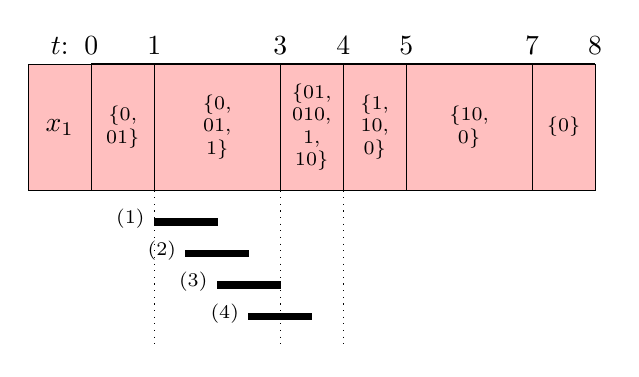
\begin{tikzpicture}[scale=0.8]
			\draw[thick] (0,-5) -- (8,-5);
			\foreach \x in {0,1,3,4,5,7,8}
			\draw (\x,-5) node[above] {\x};
			\draw (-0.5,-5) node[above] {$t$:};
			
			\draw[fill=pink] (-1,-7) rectangle (0,-5) node[midway] {$x_1$};
			\draw[fill=pink] (0,-7) rectangle (1,-5) node[midway] {\scriptsize\begin{tabular}{c}\{0,\\ 01\}\\\end{tabular}};
			\draw[fill=pink] (1,-7) rectangle (3,-5) node[midway] {\scriptsize\begin{tabular}{c}\{0,\\ 01,\\ 1\}\\\end{tabular}};
			\draw[fill=pink] (3,-7) rectangle (4,-5) node[midway] {\scriptsize{\begin{tabular}{c}\{01,\\ 010,\\ 1,\\ 10\}\\\end{tabular}}};
			\draw[fill=pink] (4,-7) rectangle (5,-5) node[midway] {\scriptsize\begin{tabular}{c}\{1,\\ 10,\\ 0\}\\\end{tabular}};
			\draw[fill=pink] (5,-7) rectangle (7,-5) node[midway] {{\scriptsize\begin{tabular}{c}\{10,\\ 0\}\\\end{tabular}}};
			\draw[fill=pink] (7,-7) rectangle (8,-5) node[midway] {{\scriptsize\begin{tabular}{c}\{0\}\\\end{tabular}}};
			
			\draw[dotted] (1,-7) -- (1,-9.5);
			\draw[dotted] (3,-7) -- (3,-9.5);
			\draw[dotted] (4,-7) -- (4,-9.5);
			
			\draw[fill=black] (1, -7.5 + 0.05) node[left]{{\scriptsize (1)}} rectangle (2, -7.5 - 0.05) ;
			\draw[fill=black] (1.5, -8 + 0.05) node[left] {{\scriptsize (2)}} rectangle (2.5, -8 - 0.05) ;
			\draw[fill=black] (2, -8.5 + 0.05) node[left] {{\scriptsize (3)}} rectangle (3, -8.5 - 0.05);
			\draw[fill=black] (2.5, -9 + 0.05) node[left] {{\scriptsize (4)}} rectangle (3.5, -9 - 0.05);
		\end{tikzpicture}
		\caption{Forward profiles of $J = [0,1)$ with respect to $x_1 \in~S$ of \cref{fig:csve}. A representative interval for each profile is shown with solid black lines below the table.}
		\label{fig:profiles}
	\end{figure}
	
	\paragraph*{Sets of Boolean Value Expressions as Bit Vectors.}
	Asynchronous products are expensive to compute.
	Our implementation relies on the observation that sets of boolean value expressions and their operations can be efficiently implemented through bit vectors.
	Intuitively, to represent such a set, we encode each element using its first bit and its length since value expressions are boolean and always destuttered.
	Moreover, to evaluate untimed operations on such sets, we only need to know the maximal lengths of the four possible types of expressions ($0 \ldots 0$, $0 \ldots 1$, $1 \ldots 0$, and $1 \ldots 1$) and whether the set contains $0$ or $1$ (to handle some edge cases).
	This is because value expressions within the same segments are completely asynchronous and the possible interleavings obtained from shorter expressions can be also obtained from longer ones.
	%This approach enables, for example, an algorithm for conjunction of sets of value expressions that runs in $O(|u| + |v|)$ time where $u$ and $v$ are the longest expressions in the two sets.
	%The same idea also applies to untimed temporal operators.
	
	%\vspace{-0.5em}
	\paragraph*{Generalization to Real-Valued Signals.}
	Our approximate distributed monitoring method, denoted \textsc{Adm}, can be extended to real-valued signals and numerical predicates.
	The key is that finite-length piecewise-constant signals take finitely many values.
	By defining $\Sigma$ as a finite alphabet of these values, we can compute atomic propositions as above.
	%%Arithmetic operations are handled by computing the asynchronous product of the signals and applying the operation letter-by-letter, transforming the results into atomic propositions via comparison with constants.
	For example, if the asynchronous product of two signals $x_1$ and $x_2$ yields $(2\cdot2\cdot3, 1\cdot0\cdot1)$, adding these letter-by-letter results in $3 \cdot 2 \cdot 4$, and comparing with $> 2$ gives $101$.
	%%Repeating this for all pairs produces the required atomic proposition.
	%\alert{This approach is called \textsc{Orig}.}
	
	We can avoid explicit computation of asynchronous products for some formulas and numerical predicates.
	Since signals are asynchronous within segments, we can compute potential value sets instead of sequences.
	This approach is called \emph{Fine}, denoted by \textsc{Adm-F}.
	Assuming signals are piecewise constant, we can avoid explicit interleaving computations by only considering how potential signal values aggregate.
	For instance, with $X_1 = \{2,3\}$ and $X_2 = \{0,1\}$, pairwise addition yields $\{2, 3, 4\}$.
	Note that \textsc{Adm-F} overapproximates traces when order matters.
	While \textsc{Adm-F} overapproximates traces when order matters, such as in $(x_1 > c_1) \until (x_2 > c_2)$, it preserves precision for formulas like $\LTLalways(x_1 + x_2 > c)$.
	The approach \emph{Coarse}, denoted \textsc{Adm-C}, abstracts \emph{Fine} by only considering extreme values, which is useful for monotonic operations where the extreme values of outputs derive from inputs.
	
	We assumed so far that the central monitor runs on a process independent of the observed agents.
	Lastly, we also consider a setting where the monitor runs on one of the observed agents.
	This approach reduces asynchrony by using the agent's local clock as a reference point for the monitor.
	We call this \emph{Relative}, denoted \textsc{Adm-Fr} or \textsc{Adm-Cr} depending on the approach it is paired with.
	We evaluate these in \cref{sec:experiments}.
	
	\paragraph*{Combining Exact and Approximate Monitoring.}
	We propose a method that combines approximate distributed monitors (\textsc{Adm}) with their exact counterparts (\textsc{Edm}) with the aim to achieve better performance while remaining precise.
	
	The approach works as follows:
	Given a distributed signal $(S,{\hb})$ and a formula $\varphi$, compute the approximate verdict $v \gets [(S,{\hb}) \models \varphi]_+$.
	If the verdict is inconclusive, i.e., $v = {\,?}$, then compute and return the exact verdict $[(S,{\hb}) \models \varphi]$, else return $v$.
	We evaluate this approach in \cref{sec:experiments}.
	
	\bgroup \color{red}
	\subsection{Online Algorithm}\label{sec:online}
	We now focus on the online setting, where the monitor does not have access to the entire signal, but it periodically reads a new \emph{portion} of the distributed signal $(S,{\hb})$ of a fixed length.
	Our goal is to describe an algorithm that computes, given a past STL formula $\varphi$, the value expressions for the satisfaction of $\varphi$ after reading each new signal portion.
	
	Let us first highlight the main difference of the online setting from the offline one.
	Unlike in the offline setting, the monitor does not know whether the current signal portion is the last one.
	After processing consecutive portions of a signal of length $d$, an edge in the next portion with a local timestamp $t' \in (d, d+\varepsilon)$ may result in new potential interleavings with the edges that have been observed in the current portion.
	As a result, if the monitor attempts to produce a verdict for the signal prefix until length $d$, it may produce an unsound verdict as it may miss potential interleavings.
	
	This problem of ``forward uncertainty'' can be avoided if the monitor only produces a verdict for the signal's prefix of length at most $d-\varepsilon$, since no edge with a local timestamp larger than $d$ can influence the verdict at time $d-\varepsilon$ with respect to the monitor's clock.
	Notice that $d-\varepsilon$ is an upper bound.
	As our approximate monitors rely on partitioning the temporal domain into fully asynchronous segments, when $d-\varepsilon$ is not a segment end point, trying to produce a conclusive verdict for it would lead to further overapproximation.
	
	Below, we detail two contrasting solutions: a \emph{naive} approach that recomputes everything from scratch after each new portion arrives, and an \emph{incremental} approach that takes advantage of the inductive computation of value expressions.
	We demonstrate these in \cref{fig:online}.
	
	\begin{figure*}
		%	\vspace{-1em}
		\centering
		\begin{subfigure}[c]{.1\textwidth}
			\centering
			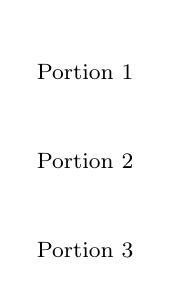
\begin{tikzpicture}[scale=0.75,>=stealth]
				% portion labels
				\node[anchor=east] at ($(-1,3.6)$) {};
				\vspace{1em}
				\node[anchor=east] at ($(-1,3)$) {\footnotesize{Portion 1}};
				\node[anchor=east] at ($(-1,1.5)$) {\footnotesize{Portion 2}};
				\node[anchor=east] at ($(-1,0)$)       {{\footnotesize Portion 3}};
			\end{tikzpicture}
		\end{subfigure}
		%	\hspace{1em}
		\begin{subfigure}[c]{.42\textwidth}
			\centering
			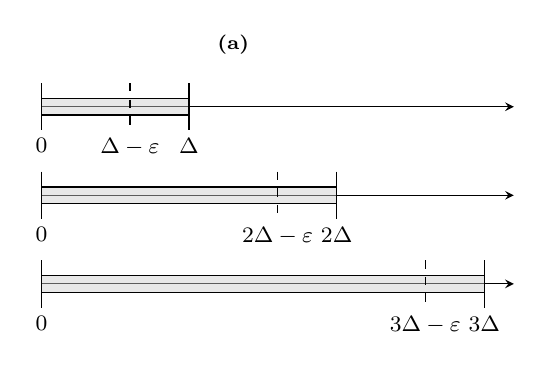
\begin{tikzpicture}[scale=0.75,
				>=stealth,
				box/.style = {fill=gray!40, draw=black, fill opacity=.45}
				]
				
				%--- handy lengths ------------------------------------------------------------
				\def\DL{2.5}        % 1·Δ  (horizontal unit)
				\def\eps{1}      % ε   (shown as small offset of the dashed line)
				\def\vsep{1.5}      % vertical separation between rows
				\def\arrowL{3*\DL+0.5}  % total arrow length (both panels)
				\def\barH{0.28}   % <── height of the grey bar
				
				%--- column anchors -----------------------------------------------------------
				\coordinate (A) at (0,0);             % left column (a)
				
				%==============================================================================
				%                               panel (a)
				%------------------------------------------------------------------------------
				\scriptsize
				\node at ($(A)+(1.5*\DL,2.1*\vsep+0.9)$) {\textbf{(a)}};
				\footnotesize
				
				% portion labels
				%			\node[anchor=east] at ($(A)+(-0.8,2*\vsep)$) {Portion 1};
				%			\node[anchor=east] at ($(A)+(-0.8,1*\vsep)$) {Portion 2};
				%			\node[anchor=east] at ($(A)+(-0.8,0)$)       {Portion 3};
				
				% -- row 1 -------------------------------------------------
				\draw[->] ($(A)+(0.5,2*\vsep)$) -- ++(\arrowL,0);
				\path ($(A)+(0.5,2*\vsep)$) coordinate (s1a);
				\filldraw[box] ($(s1a)+(0,-\barH/2)$) rectangle ++(\DL,\barH);
				\draw[solid] ($(s1a)+(0,0.4)$) -- ++(0,-0.8);
				\draw[solid] ($(s1a)+(\DL,0.4)$) -- ++(0,-0.8);
				\draw[dashed] ($(s1a)+(\DL-\eps,0.4)$) -- ++(0,-0.8);
				\node[below]  at ($(s1a)+(0,     -0.4)$) {$0$};
				\node[below]  at ($(s1a)+(\DL-\eps, -0.4)$) {$\Delta-\varepsilon$};
				\node[below]  at ($(s1a)+(\DL,      -0.4)$) {$\Delta$};
				
				% -- row 2 -------------------------------------------------
				\draw[->] ($(A)+(0.5,1*\vsep)$) -- ++(\arrowL,0);
				\path ($(A)+(0.5,1*\vsep)$) coordinate (s2a);
				\filldraw[box] ($(s2a)+(0,-\barH/2)$) rectangle ++(2*\DL,\barH);
				\draw[dashed] ($(s2a)+(2*\DL-\eps,0.4)$) -- ++(0,-0.8);
				\draw[solid] ($(s2a)+(0,0.4)$) -- ++(0,-0.8);
				\draw[solid] ($(s2a)+(2*\DL,0.4)$) -- ++(0,-0.8);
				\node[below]  at ($(s2a)+(0,     -0.4)$) {$0$};
				\node[below]  at ($(s2a)+(2*\DL-\eps,-0.4)$) {$2\Delta-\varepsilon$};
				\node[below]  at ($(s2a)+(2*\DL,     -0.4)$) {$2\Delta$};
				
				% -- row 3 -------------------------------------------------
				\draw[->] ($(A)+(0.5,0)$)       -- ++(\arrowL,0);
				\path ($(A)+(0.5,0)$) coordinate (s3a);
				\filldraw[box] ($(s3a)+(0,-\barH/2)$) rectangle ++(3*\DL,\barH);
				\draw[dashed] ($(s3a)+(3*\DL-\eps,0.4)$) -- ++(0,-0.8);
				\draw[solid] ($(s3a)+(0,0.4)$) -- ++(0,-0.8);
				\draw[solid] ($(s3a)+(3*\DL,0.4)$) -- ++(0,-0.8);
				\node[below]  at ($(s3a)+(0,     -0.4)$) {$0$};
				\node[below]  at ($(s3a)+(3*\DL-\eps,-0.4)$) {$3\Delta-\varepsilon$};
				\node[below]  at ($(s3a)+(3*\DL,     -0.4)$) {$3\Delta$};
			\end{tikzpicture}
		\end{subfigure}
		\hspace{1em}
		\begin{subfigure}[c]{.42\textwidth}
			\centering
			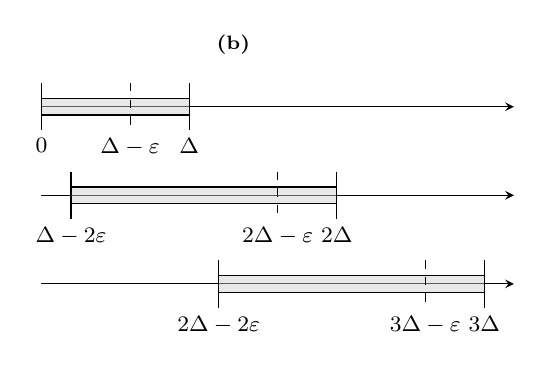
\begin{tikzpicture}[scale=0.75,
				>=stealth,
				box/.style = {fill=gray!40, draw=black, fill opacity=.45}
				]
				
				%--- handy lengths ------------------------------------------------------------
				\def\DL{2.5}        % 1·Δ  (horizontal unit)
				\def\eps{1}      % ε   (shown as small offset of the dashed line)
				\def\vsep{1.5}      % vertical separation between rows
				\def\arrowL{3*\DL+0.5}  % total arrow length (both panels)
				\def\barH{0.28}   % <── height of the grey bar
				
				%--- column anchors -----------------------------------------------------------
				\coordinate (B) at (0,0);             % left column (a)
				
				%==============================================================================
				%                               panel (b)
				%------------------------------------------------------------------------------
				\scriptsize
				\node at ($(B)+(1.5*\DL,2.1*\vsep+0.9)$) {\textbf{(b)}};
				\footnotesize 	
				
				% -- row 1 -------------------------------------------------
				\draw[->] ($(B)+(0.5,2*\vsep)$) -- ++(\arrowL,0);
				\path ($(B)+(0.5,2*\vsep)$) coordinate (s1b);
				\filldraw[box] ($(s1b)+(0,-\barH/2)$) rectangle ++(\DL,\barH);
				\draw[dashed] ($(s1b)+(\DL-\eps,0.4)$) -- ++(0,-0.8);
				\draw[solid] ($(s1b)+(0,0.4)$) -- ++(0,-0.8);
				\draw[solid] ($(s1b)+(\DL,0.4)$) -- ++(0,-0.8);
				\node[below]  at ($(s1b)+(0,-0.4)$) {$0$};
				\node[below]  at ($(s1b)+(\DL-\eps,-0.4)$) {$\Delta-\varepsilon$};
				\node[below]  at ($(s1b)+(\DL,     -0.4)$) {$\Delta$};
				
				% -- row 2 -------------------------------------------------
				\draw[->] ($(B)+(0.5,1*\vsep)$) -- ++(\arrowL,0);
				\path ($(B)+(0.5+\DL-2*\eps,1*\vsep)$) coordinate (s2b);
				\filldraw[box] ($(s2b)+(0,-\barH/2)$) rectangle ++(\DL+2*\eps,\barH);
				\draw[dashed] ($(s2b)+(\DL+\eps,0.4)$) -- ++(0,-0.8);
				\draw[solid] ($(s2b)+(0,0.4)$) -- ++(0,-0.8);
				\draw[solid] ($(s2b)+(\DL+2*\eps,0.4)$) -- ++(0,-0.8);
				\node[below] at ($(s2b)+(0,         -0.4)$) {$\Delta-2\varepsilon$};
				\node[below] at ($(s2b)+(\DL+\eps,-0.4)$) {$2\Delta-\varepsilon$};
				\node[below] at ($(s2b)+(\DL+2*\eps,     -0.4)$) {$2\Delta$};
				
				% -- row 3 -------------------------------------------------
				\draw[->] ($(B)+(0.5,0)$)       -- ++(\arrowL,0);
				\path ($(B)+(0.5+2*\DL-2*\eps,0)$) coordinate (s3b);
				\filldraw[box] ($(s3b)+(0,-\barH/2)$) rectangle ++(\DL+2*\eps,\barH);
				\draw[dashed] ($(s3b)+(\DL+\eps,0.4)$) -- ++(0,-0.8);
				\draw[solid] ($(s3b)+(0,0.4)$) -- ++(0,-0.8);
				\draw[solid] ($(s3b)+(\DL+2*\eps,0.4)$) -- ++(0,-0.8);
				\node[below] at ($(s3b)+(0,         -0.4)$) {$2\Delta-2\varepsilon$};
				\node[below] at ($(s3b)+(\DL+\eps,-0.4)$) {$3\Delta-\varepsilon$};
				\node[below] at ($(s3b)+(\DL+2*\eps,     -0.4)$) {$3\Delta$};
			\end{tikzpicture}
		\end{subfigure}
		\vspace{1ex}
		\caption{\bgroup \color{red}
			Two contrasting approaches to online monitoring with a sampling period of $\Delta$ and a maximum clock skew of $\varepsilon$. The signal (solid arrows) become available incrementally. As new portions of the signal arrive, the monitor stores some part of it (gray boxes around solid arrows). In both approaches, after receiving the $i$th signal portion, the monitor can give a conclusive verdict for time at most $i\Delta-\varepsilon$ with respect to its local clock (dashed lines).
			\textbf{(a)} The \emph{naive} monitor stores the entire signal it has read so far and computes its verdict from scratch each time a new portion arrives.
			\textbf{(b)} The \emph{incremental} monitor stores only the current portion it receives and a fraction of the previous portion sufficient to correctly compute the value expressions for the current one. Here, we assume the monitor is able to produce a verdict for time $i\Delta-\varepsilon$ for every $i \geq 1$. Since no edges with timestamps earlier than $i\Delta-2\varepsilon$ can influence the segmentation between $i\Delta-\varepsilon$ and $i\Delta$, the monitor can drop from its memory the signal's prefix of length $i\Delta-2\varepsilon$. \egroup\label{fig:online}}
		%	\vspace{1em}
	\end{figure*}
	
	
	\paragraph*{Naive algorithm.}
	The \emph{naive} strategy, denoted \textsc{Adm-Naive}, stores the entire history of $(S,{\hb})$ (i.e., all the portions observed so far) and runs the offline algorithm we presented in \cref{sec:offline} whenever a new portion is received.
	
	As we discussed above, when there is forward uncertainty, for a signal of length $d$, the monitor can only give a conclusive verdict for its prefix of length at most $d-\varepsilon$.
	To compute this conclusive verdict, the monitor finds in the signal's canonical segmentation the latest segment whose right end point is less than or equal to $d-\varepsilon$.
	Since no future edges can influence the potential interleavings in this segment, the monitor processes the signal until the end of this segment to produce its verdict.
	%To compute this conclusive verdict, the monitor needs to take into account two scenarios: one in which the edges with local timestamps in $(d-2\varepsilon, d)$ happens before time $d-\varepsilon$ with respect to the monitor's clock, and another in which they happen after $d-\varepsilon$.
	%The ``before'' scenario is handled by including the value expressions of these edges in the computation, and the ``after'' scenario by taking their prefixes.
	
	More specifically, \textsc{Adm-Naive} follows the steps below:
	\begin{enumerate}[label*=\arabic*.]
		\item Initialize $(S,{\hb})$ as an empty signal.
		\item Repeat for $i \geq 1$:
		\begin{enumerate}[leftmargin=5pt,label*=\arabic*]
			\item Append the new signal portion $(S_i,{\hb}_i)$ to $(S,{\hb})$ and let $d$ be the length of $(S,{\hb})$.
			\item Compute the canonical segmentation $G_S$.
			\item Find the segment $J = [a, a') \in G_S$ with the largest $a' \leq d-\varepsilon$.
			%		\item For every segment $I \in G_S$ whose right end point is at most $a'$, compute $\llbracket (S, {\hb}), I \models \varphi \rrbracket$ inductively.
			\item Compute and output  $\llbracket (S, {\hb}), i \models \varphi \rrbracket_{\textit{naive}} \defeq \llbracket (S, {\hb}), J \models \varphi \rrbracket$.
		\end{enumerate}
	\end{enumerate}
	%\begin{enumerate}[label*=\arabic*.]
	%	\item Initialize $(S,{\hb})$ as an empty signal.
	%	\item Repeat for $i \geq 1$:
	%	\begin{enumerate}[leftmargin=5pt,label*=\arabic*]
		%		\item Append the new signal portion $(S_i,{\hb}_i)$ to $(S,{\hb})$ and let $d$ be the length of $(S,{\hb})$.
		%		\item Compute the canonical segmentation $G_S$.
		%		\item For every signal $x \in S$ and segment $I = [a, a') \in G_S$, compute the set of value expressions $\gamma(x,I)$ as usual, and if $d-\varepsilon < a'$ then update it as $\pfx(\gamma(x,I))$.
		%		\item For every segment $I \in G_S$, compute $\llbracket (S, {\hb}), I \models \varphi \rrbracket$ inductively.
		%		\item Output $\llbracket (S, {\hb}), i \models \varphi \rrbracket_{\textit{naive}} \defeq \llbracket (S, {\hb}), J \models \varphi \rrbracket$ where $J = [b,b') \in G_S$ is the segment such that $d - \varepsilon = b'$, if such a segment exists, and $d - \varepsilon \in J$ otherwise.
		%	\end{enumerate}
	%\end{enumerate}
	Thanks to the soundness of our offline monitoring algorithm (\cref{cl:algo}), \textsc{Adm-Naive} is sound.
	The computation of value expression sets, i.e., the $\gamma$ function, already captures the uncertainty due to clock skew, and the monitor considers only a prefix that cannot be affected by future edges.
	%At Step 2.3 above, by prefixing the value expressions only on the segments that end after $d-\varepsilon$, we capture the uncertainty on whether the signal ends here or not.
	Despite its immediate soundness, both time and memory consumption of \textsc{Adm-Naive} per portion grow with the signal length, which is impractical for long-running systems.
	
	\paragraph*{Incremental algorithm.}
	The \emph{incremental} approach, \textsc{Adm-Incr}, avoids global recomputation and processes each new portion once by taking advantage of the inductive computation of value expressions, which we presented in \cref{sec:offline}.
	For every subformula $\psi$ of $\varphi$ and every new portion, the monitor maintains a summary capturing the potential truth values of $\psi$.
	%For every subformula $\psi$ of $\varphi$ and every new portion, the monitor maintains the set of value expressions for the satisfaction of $\psi$ in the portion and a summary capturing the potential truth values of $\psi$ at the end of the portion.
	When a new portion arrives, these summaries are used to inductively compute the new value expressions and the summaries are updated accordingly.
	
	As expected, \textsc{Adm-Incr} handles the problem of forward uncertainty exactly as \textsc{Adm-Naive} does, which powers the inductive computation.
	However, for \textsc{Adm-Incr} there is a dual ``backward uncertainty'' problem:
	Suppose we have an incremental monitor for an untimed past STL formula $\varphi$ and it receives new signal portions with a period of $\Delta > 0$.
	It processes the initial portion the same as \textsc{Adm-Naive}, so its verdict reflects the satisfaction of $\varphi$ at the end of the latest segment $J = [a, a')$ with $a' \leq \Delta - \varepsilon$.
	Although this segment could serve as a synchronization point, the incremental approach leads to the question of how much of the past signal the monitor should keep in memory.
	
	The following observation settles this question:
	The verdicts of the previous portion can be carried forward correctly only if the segmentation between $a'$ and $\Delta$ is preserved.
	It means that the monitor can drop from its memory the edges that cannot influence the segmentation between $a'$ and $\Delta$.
	Therefore, it suffices to consider the edges with local timestamps at least $a' - \varepsilon$ and use the previous portion's verdict to compute the next portion's verdict inductively.
	This establishes that the monitor needs to store (i)~the observations from the previous portion with timestamps greater than or equal to $a' - \varepsilon$, and (ii)~the verdict in segment $J$ for every subformula of $\varphi$.
	
	%As expected, \textsc{Adm-Incr} handles the problem of forward uncertainty exactly as \textsc{Adm-Naive} does.
	%However, for \textsc{Adm-Incr} there is a dual ``backward uncertainty'' problem:
	%Suppose we have an incremental monitor for an untimed past STL formula $\varphi$ and it receives new signal portions with a period of $\Delta > 0$.
	%It processes the initial portion the same as \textsc{Adm-Naive}, so its verdict reflects the satisfaction of $\varphi$ until time $\Delta - \varepsilon$ with respect to its local clock.
	%The next portion has local timestamps in the range $[\Delta, 2\Delta)$.
	%The edges with local timestamps in $[\Delta - \varepsilon, \Delta)$ may have happened before time $\Delta - \varepsilon$ with respect to the monitor's local clock, which leads to the question of how they should be handled and how much of the past signal the monitor should keep in memory.
	%
	%The following observation settles these questions:
	%Whether these edges happen before or after time $\Delta - \varepsilon$ has been already considered while processing the previous portion.
	%Therefore, it suffices to treat these edges as if they happen after $\Delta - \varepsilon$ and use the previous portion's verdict to compute the next portion's verdict inductively.
	%This establishes that the monitor at least needs to store (i)~the observations from the previous portion with timestamps greater than or equal to $\Delta - \varepsilon$, and (ii)~the previous portion's verdict for every subformula of $\varphi$.
	%However, this may not be enough: if there is an edge with timestamp exactly $\Delta - \varepsilon$, the monitor would treat the current segment as if it's initial value is certain, while depending on whether this edge happens before or after $\Delta - \varepsilon$ with respect to the monitor's clock changes the signal's initial value on the new portion.
	%To distinguish whether there is such an edge, we let $\delta > 0$ be a constant much smaller than $\varepsilon$ and $\Delta$, and require the monitor to store the observations from the previous portion with timestamps greater than or equal to $\Delta - \varepsilon - \delta$ instead.
	
	In the above explanation, we assumed an untimed past STL formula.
	For timed formulas, the monitor may need to store signal values further in the past because of the sliding window computation involved in the inductive evaluation of timed since (\cref{fig:timedEval}).
	Given a timed past STL formula $\varphi$, we define its \emph{memory horizon} $M(\varphi)$ inductively as follows:
	\begin{align*}
		M(p) &= 0 \\
		M(\lnot \varphi) &= M(\varphi) \\
		M(\varphi_1 \land \varphi_2) &= \max(M(\varphi_1), M(\varphi_2))\\
		M(\varphi_1 \since_I \varphi_2) &= h(I) + \max(M(\varphi_1), M(\varphi_2))
	\end{align*}
	where we let $h(I) = \inf I$ if $\sup I = \infty$ and $h(I) = \sup I$ otherwise.
	More specifically, \textsc{Adm-Incr} with the sampling period $\Delta > 0$ follows the steps below:
	\begin{enumerate}[label*=\arabic*.]
		\item Initialize $(S,{\hb})$ as an empty signal, $V = \{0\}$ as a summary of the previous portion's verdict, and $v = 0$.
		\item Repeat for $i \geq 1$:
		\begin{enumerate}[leftmargin=5pt,label*=\arabic*]
			\item Remove the prefix of $(S,{\hb})$ of length $\max(0, (i-1)\Delta - M(\varphi) - 2\varepsilon)$ and append the new signal portion $(S_i,{\hb}_i)$ to $(S,{\hb})$.
			\item Compute the canonical segmentation $G_S$ and remove the segments whose right end point is at most $v$.
			\item Let $\hat{I} = [-1, v)$ be an imaginary segment and $\llbracket (S, {\hb}), \hat{I} \models \psi \rrbracket \defeq V$ for every subformula $\psi$ of $\varphi$.
			\item Find the segment $J = [a, a') \in G_S$ with the largest $a' \leq i\Delta-\varepsilon$.
			\item Compute and output $\llbracket (S, {\hb}), i \models \varphi \rrbracket_{\textit{incr}} \defeq \llbracket (S, {\hb}), J \models \varphi \rrbracket$.
			\item Let $V = \last(\llbracket (S, {\hb}), J \models \varphi \rrbracket)$ and $v = a'$.
		\end{enumerate}
	\end{enumerate}
	%\begin{enumerate}[label*=\arabic*.]
	%	\item Initialize $(S,{\hb})$ as an empty signal and $V = \{0\}$ as a summary of the previous portion's verdict.
	%	\item Repeat for $i \geq 1$:
	%	\begin{enumerate}[leftmargin=5pt,label*=\arabic*]
		%		\item Remove the prefix of $(S,{\hb})$ of length $\Delta - H(\varphi) - \varepsilon - \delta$  and append the new signal portion $(S_i,{\hb}_i)$ to $(S,{\hb})$.
		%		\item Compute the canonical segmentation $G_S$.
		%		\item Let $\hat{I} = [-1, x)$ be an imaginary segment where $x$ is the left end point of the first segment in $G_S$, and $\llbracket (S, {\hb}), \hat{I} \models \varphi \rrbracket \defeq V$.
		%		\item For every signal $x \in S$ and segment $I = [a, a') \in G_S$, compute the set of value expressions $\gamma(x,I)$ as usual, and if $i\Delta - \varepsilon < a'$ then update it as $\pfx(\gamma(x,I))$.
		%		\item For every segment $I \in G_S$, compute $\llbracket (S, {\hb}), I \models \varphi \rrbracket$ inductively.
		%		\item Output $\llbracket (S, {\hb}), i \models \varphi \rrbracket_{\textit{incr}} \defeq \llbracket (S, {\hb}), J \models \varphi \rrbracket$ where $J = [b,b') \in G_S$ is the segment such that $i\Delta - \varepsilon = b'$, if such a segment exists, and $i\Delta - \varepsilon \in J$ otherwise, and update $V = \last(\llbracket (S, {\hb}), i \models \varphi \rrbracket_{\textit{incr}})$.
		%	\end{enumerate}
	%\end{enumerate}
	
	Intuitively, \textsc{Adm-Incr} simulates \textsc{Adm-Naive} portion by portion.
	For an untimed formula, after processing the $(i-1)$st portion it keeps (i) the suffix of the signal starting at $(i-1)\Delta - 2\varepsilon$ and (ii) for every subformula of $\varphi$ the verdict that the offline monitor already produced for the prefix finishing at the latest segment that ends before $(i-1)\Delta - \varepsilon$ together with its right end point.
	When the $i$th portion arrives, \textsc{Adm-Incr} replaces older data with an imaginary segment that stores the previous portion's verdicts, appends the new portion, and then runs exactly the same inductive rules that the offline algorithm would apply to the full signal.
	Because the uncertain edges in the last $2\varepsilon$ time units are still present, the part of the segmentation between the last verdict's timestamp and $i\Delta$ is preserved.
	Moreover, the summary segment supplies the correct past truth values.
	Therefore, every intermediate value expression, and hence the final verdict at the end of the portion, is identical in \textsc{Adm-Naive} and \textsc{Adm-Incr}.
	%Repeating this argument for every $i$ shows that the two algorithms output the same verdict stream.
	
	\begin{theorem} \label{cl:algoOnline}
		The outputs of \textsc{Adm-Naive} and \textsc{Adm-Incr} coincide after every new signal portion.
		Formally, consider a distributed signal $(S,{\hb})$ that incrementally becomes available and a past STL formula $\varphi$.
		Then, for every $i \geq 1$, the following equality holds:
		\begin{align*}
			\llbracket (S, {\hb}), i \models \varphi \rrbracket_{\textit{naive}} = \llbracket (S, {\hb}), i \models \varphi \rrbracket_{\textit{incr}}
		\end{align*}
	\end{theorem}
	\begin{proof}[\normalsize Proof.]
		\normalsize
		We prove the statement by induction over the number $i \geq 1$ of signal portions that have been processed.
		
		\subparagraph*{Base case ($i = 1$).}
		Since the inductive evaluation assumes that formulas are violated when signals are undefined, initializing $V = \{0\}$ and $v=0$ in \textsc{Adm-Incr} guarantees that \textsc{Adm-Incr} and \textsc{Adm-Naive} behave exactly the same.
		
		
		\subparagraph*{Induction step.}
		Assume that after processing the first $i$ portions the two algorithms have
		produced identical verdicts, i.e., $ \llbracket (S,\hb), i \models \varphi \rrbracket_{\textit{naive}} = \llbracket (S,\hb), i \models \varphi \rrbracket_{\textit{incr}}$.
		
		When the $(i+1)$st portion $(S_{i+1},\hb_{i+1})$ arrives, \textsc{Adm-Naive} concatenates it with the entire previous signal prefix and obtains a longer signal
		Let us denote this signal by $\sigma_{i+1}$.
		In contrast, \textsc{Adm-Incr} discards the part of the prefix that ends before $i\Delta - H(\varphi) - 2\varepsilon$, which guarantees that all edges that may still interact with future edges are retained, and inserts a summary segment
		$\hat{I}$ and for every subformula $\psi$ of $\varphi$ lets $\llbracket (S,\hb), \hat{I} \models \psi \rrbracket = \llbracket (S,\hb), i \models \psi \rrbracket_{\textit{incr}}$, which, by induction hypothesis, coincides with $\llbracket (S,\hb), i \models \psi \rrbracket_{\textit{naive}}$.
		Let us denote the resulting signal by $\sigma_{i+1}'$.
		
		We claim that for every subformula $\psi$ of $\varphi$ and for every segment $I$ of the canonical segmentation of $\sigma_{i+1}$ that lies strictly to the right of $\hat{I}$, we have $\llbracket \sigma_{i+1}, I \models \psi\rrbracket = \llbracket \sigma_{i+1}', I \models \psi \rrbracket$.
		To see why this holds, observe that (i) these parts of the segmentations coincide because \textsc{Adm-Incr} takes into account all the edges in the past that might have an effect here, (ii) the value expressions of the atomic propositions also coincide for the same reason, and (iii) both monitors run exactly the same inductive rules (given in \cref{sec:offline}, \cref{fig:eval,fig:timedEval}).
		These rules evaluate a subformula on a segment $I$ from the value expressions of atomic propositions for the current segment $I$ and the value expression set already computed for the immediate predecessor segment $I'$.
		By the induction hypothesis, the verdicts stored for $\hat{I}$ coincides with that of the prefix of $\sigma_{i+1}$ that is discarded in $\sigma_{i+1}'$, so the computed value expression sets for $I'$ are also equal.
		Therefore, the inductive rules yield identical results on $I$ for $\sigma_{i+1}$ and $\sigma_{i+1}'$.
		Finally, since the latest segment $J$ in the canonical segmentation whose right end point is less than or equal to $(i+1)\Delta - \varepsilon$ also lies strictly to the right of $\hat{I}$, we conclude
		$$\llbracket (S,\hb), i+1 \models \varphi \rrbracket_{\textit{naive}} = \llbracket (S,\hb), i+1 \models \varphi \rrbracket_{\textit{incr}}.$$
	\end{proof}
	
	We evaluate the performance of \textsc{Adm-Incr} against \textsc{Adm-Naive} in \cref{sec:experiments}.
	\egroup
	
	
	
	
	
	
	\section{Experimental Evaluation} 
	\label{sec:experiments}
	
	%This section presents the research questions and the experiments we conducted and analyzed to validate our approximate distributed monitoring approach.
	
	%\subsection{Research Questions}
	
	We seek answers to the following research questions (RQs):
	%\vspace{-0.25em}
	\begin{resq}[What is the tradeoff between the efficiency and the accuracy of approximate distributed monitors?]
		The approximate distributed monitoring comes with a price in terms of the loss of accuracy.
		We want to understand the tradeoff between the potential speedups that an approximate distributed monitor can achieve when compared to its exact counterpart and the consequent loss in accuracy due to the approximations.
		We would also like to identify the classes of signals and properties for which this tradeoff is effective. 
	\end{resq}
	%\vspace{-0.75em}
	\begin{resq}[Can the combination of approximate and exact distributed monitors increase efficiency while preserving accuracy?]
		We are interested in evaluating whether a smart, combined use of approximate and exact distributed monitors can still bring improvements in monitoring efficiency while guaranteeing the accuracy of the monitoring verdicts. 
	\end{resq}
	\bgroup \color{red}
	\begin{resq}[How scalable are online incremental monitors?]
		The offline monitors can be naively used for online monitoring, which comes with immediate soundness but computational overhead due to redundant computation and using memory carelessly.
		The alternative, incremental monitoring approach aims to address these issues.
		We want to understand to which degree the incremental approach achieves this goal and scales to scenarios with high-frequency sampling and large clock skew.
	\end{resq}
	\egroup
	
	\begin{table*}[t]
		\centering
		%	\scalebox{0.88}{
			\begin{tabular}{|l|l|}
				\hline
				Subject & STL formula(s) \\
				\hline
				%			RG & $\varphi_1 =\LTLg (p \wedge q)$ \,\,\,\,\,\, $\varphi_2 = \LTLg (p \Rightarrow \LTLf q)$ \,\,\,\,\,\, $\varphi_3 = \LTLg (p \Rightarrow \LTLf_{[0,1)} q)$ \\
				%			   & $\varphi_4 = \LTLg (p \lor q)$ \,\,\,\,\,\,  $\varphi_5 = p \until q$ \,\,\,\,\,\, $\varphi_6 = \LTLg (p \Rightarrow \LTLf_{[0,2)} q)$ \\
				RG (offline) & $\varphi_1 =\LTLg (p \wedge q)$ \,\,\,\,\,\,\,\,\,\,\,\,\,\,\, $\varphi_2 =\LTLg (p \lor q)$ \,\,\,\,\,\,\,\,\,\,\,\,\,\,\,\,\,\,\,\,\,\,\,\,\, $\varphi_3 = p \until q$ \\
				& $\varphi_4 = \LTLg (p \Rightarrow \LTLf q)$  \,\,\,\,\,\,  $\varphi_5 = \LTLg (p \Rightarrow \LTLf_{[0,1)} q)$ \,\,\,\,\,\, $\varphi_6 = \LTLg (p \Rightarrow \LTLf_{[0,2)} q)$ \\
				RG (online) & $\psi_1 =\LTLsquareminus (p \wedge q)$ \,\,\,\,\,\,\,\,\,\,\,\,\,\,\, $\psi_2 =\LTLsquareminus (p \lor q)$ \,\,\,\,\,\,\,\,\,\,\,\,\,\,\,\,\,\,\,\,\,\,\,\,\, $\psi_3 = p \since q$ \\
				& $\psi_4 = \LTLsquareminus (p \Rightarrow \LTLdiamondminus q)$  \,\,\,\,\,\,  $\psi_5 = \LTLsquareminus (p \Rightarrow \LTLdiamondminus_{[0,1)} q)$ \,\,\,\,\,\, $\psi_6 = \LTLsquareminus (p \Rightarrow \LTLdiamondminus_{[0,2)} q)$ \\
				%& $\varphi_1$ & $\LTLg (p \wedge q)$ & \multirow{ 5}{*}{untimed} \\
				%& $\varphi_2$ & $\LTLf (p \vee q)$ & \\
				%& $\varphi_3$ & $\LTLg (p \vee q)$ & \\
				%& $\varphi_4$ & $\LTLf (p \wedge q)$ & \\
				%& $\varphi_5$ & $p \until q$ & \\
				%			\hline
				WT & $\varphi_{\text{WT}} = \LTLg \left(\sum_{i=1}^{n} x_i  > c\right)$  \\
				%			\hline
				SD & $\varphi_{\text{SD}} = \bigwedge_{1 \leq i \neq j \leq n} \LTLg \left( \sqrt{(x_i-x_j)^2 + (y_i-y_j)^2 + (z_i-z_j)^2} > c \right)$   \\
				\hline
			\end{tabular}%}
		\caption{STL specifications used in the experiments.}
		%	\vspace{-3em}
		\label{tab:spec} 
	\end{table*}
	
	\subsection{Experimental Setup}
	
	\paragraph*{Distributed Monitors.}
	In our study, we compare our approximate distributed monitoring (\textsc{Adm}) approach and its variants to an exact distributed monitoring approach (\textsc{Edm}).\footnote[1]{The code is available at \url{https://github.com/egesarac/ApxDistMon}.}
	For \textsc{Edm}, we take a variant of the distributed monitoring procedure from~\cite{MomtazAB23} that allows to evaluate STL specifications over distributed traces using SMT-solving.
	Originally, that procedure assumes that input signals are polynomial continuous functions.
	We adapt the SMT-based approach to consider input signals as piecewise-constant signals to make a consistent comparison with \textsc{Adm}.
	We note that the passage from the polynomial continuous to piecewise-constant input signals reduces the efficiency of the SMT-based monitors.
	We also observe that the SMT-based monitors from~\cite{MomtazAB23} can split the input trace into multiple segments and evaluate the specification incrementally, segment-by-segment, allowing early termination of the monitor in some cases.
	Since the focus of this comparison is purely on the offline monitoring, we also use the exact monitors without their incremental mode.
	%We use the abbreviation \textsc{Edm} to denote the variant of the exact SMT-based distributed monitors used in this study.
	
	%\vspace{-0.35em}
	\paragraph*{Experimental Subjects.}
	To answer our research questions, we use (1) a \emph{random generator (RG)} of distributed traces, (2) a \emph{water tank (WT)} case study, and (3) a \emph{swarm of drones (SD)} case study.  
	%
	\emph{The random generator (RG)} uses uniform distribution to generate distributed traces, in which the user can control the duration $d$ of the trace, as well as the $\varepsilon$ bound on the uncertainty at which the events happen.
	\emph{Water tank (WT)} model is a SimuLink model of a hybrid high pressure water distribution system consisting of two water tanks. Inlet pipes connect each water tank to an external source, and outlet pipes distribute high pressure water that is regulated by valves.
	Each valve is operated by a controller that samples the outflow pressure at 20Hz using its local clock. Our model is a simplified emulation of the Refueling Water Storage Tanks (RWST) module of an Emergency Core Cooling System (ECCS) of a Pressurized Water Reactor Plant~\cite{USNRCPWR}.
	\emph{Swarm of drones (SD)} model is generated using a path planning software, Fly-by-Logic~\cite{PantAM17CCTA}. Here, a swarm of drones perform various reach-avoid missions, while securing objectives such as reaching a goal within a deadline, avoiding obstacles and collisions. The path planner finds the most robust trajectory using a temporal logic robustness optimizer. These trajectories are sampled at 20Hz.
	Note that the actual values of clock skew are less important than the fact that when clock skew exceeds the sampling interval, we encounter the problem of uncertainty.
	

	
	%\vspace{-0.4em}
	\paragraph*{Specifications.}
	Table~\ref{tab:spec} shows the STL specifications that we use to evaluate our experimental subjects.
	For offline monitoring, specifications $\varphi_{1}$ to $\varphi_{6}$ are monitored against the distributed traces created by the random generator and represent different classes and fragments of Boolean-valued temporal formulas.
	The specification $\varphi_1$ is an LTL formula in which both the outer temporal operator ($\LTLg$) and the inner Boolean operator ($\wedge$) are conjunctive.
	The specification $\varphi_2$ combines conjunctive $(\LTLg)$ and disjunctive ($\lor$) operators, and $\varphi_3$ is the usual until operator.
	The remaining three formulas are the common response formulas, which also combine conjunctive $(\LTLg)$ and disjunctive $(\LTLf, \Rightarrow)$ operators: $\varphi_4$ is the usual LTL variant, $\varphi_5$ and $\varphi_6$ add a bounded real-time response requirement to the previous specification, where the bound of $\varphi_5$ is tighter than that of $\varphi_6$.
	\textcolor{red}{For online monitoring, we use the past-time variants $\psi_1$ to $\psi_6$ of the formulas described above.}
	The specification $\varphi_{WT}$ associated to the water tank case study is an STL formula in which a sum of signals originating from different agents is compared to a constant. Finally, the specification $\varphi_{SD}$ defines a mutual separation property over a swarm of drones, requiring more sophisticated arithmetic operations on signals originating from different agents.
	
	%\begin{table}[t]
	%\centering
	%\scalebox{0.85}{
		%\begin{tabular}{|l|l|l|l|}
		%\hline
		%Subject & Spec ID & STL formula \\
		%\hline
		%\multirow{3}{*}{RG}
		%& $\varphi_1$ & $\LTLg (p \wedge q)$  \\
		%& $\varphi_2$ & $\LTLg (p \Rightarrow \LTLf q)$ \\
		%& $\varphi_3$ & $\LTLg (p \Rightarrow \LTLf_{[0,1)} q)$  \\
		%%& $\varphi_1$ & $\LTLg (p \wedge q)$ & \multirow{ 5}{*}{untimed} \\
		%%& $\varphi_2$ & $\LTLf (p \vee q)$ & \\
		%%& $\varphi_3$ & $\LTLg (p \vee q)$ & \\
		%%& $\varphi_4$ & $\LTLf (p \wedge q)$ & \\
		%%& $\varphi_5$ & $p \until q$ & \\
		%\hline
		%WT & $\varphi_{\text{WT}}$ & $\LTLg \left(\sum_{i=1}^{n} x_i  > c\right)$  \\
		%SD & $\varphi_{\text{SD}}$ & $\bigwedge_{1 \leq i \neq j \leq n} \LTLg \left( \sqrt{(x_i-x_j)^2 + (y_i-y_j)^2 + (z_i-z_j)^2} > c \right)$   \\
		%\hline
		%\end{tabular}}
		%\caption{STL specifications used in the experiments.}
		%\vspace{-3em}
		%\label{tab:spec} 
		%\end{table}
		
		%\vspace{-0.4em}
		\paragraph*{Computing Platform.}
		We used a laptop with Ubuntu 24.04, an AMD Ryzen 7 4800HS CPU at 2.90GHz clock rate, and 16GB of RAM.
		\textsc{Adm} is implemented in C++ and compiled using \texttt{g++} version 13.2.0 with the optimization flag \texttt{-O3} enabled, and \textsc{Edm} invokes the SMT-solver Z3 \cite{MouraB08} and is based on \cite{MomtazAB23}.
		
		\subsection{Discussion}	
		
		%\vspace{-0.3em}
		\paragraph*{Random Generator, Offline Monitoring.}
		Figure~\ref{fig:rgresults} summarizes the results of evaluating specifications $\varphi_1$ to $\varphi_6$ against distributed traces from RG.
		The first column in the figure depicts a heatmap where cells show the speedup of \textsc{Adm} compared to \textsc{Edm} when evaluating the formula on the given distributed trace with duration $d$ and uncertainty bound $\varepsilon$.
		The second column shows a heatmap where every cell shows the percentage of \emph{false positives} (FP) introduced by \textsc{Adm}, where \textsc{Adm} evaluates to inconclusive when the \textsc{Edm} (real) verdict is true or false.
		Finally, the third column depicts a heatmap, where each cell estimates the achieved speedup when combining \textsc{Adm} with \textsc{Edm}, compared to using only \textsc{Edm}.
		
		
		We see that \textsc{Adm} consistently achieves speedups of \emph{several orders of magnitude} 
		compared to the \textsc{Edm} approach.
		The speedups range from several thousands to almost 60 thousand times, regardless of the considered specification, the duration $d$ of the trace, or the uncertainty bound $\varepsilon$.
		These speedups and are the highest for long signals with low uncertainty bounds.
		The price paid in terms of accuracy highly depends on the type of specification and the uncertainty bounds.
		For example, \textsc{Adm} is very accurate when monitoring the property $\varphi_1$ in which both the temporal and the combinatorial operators are conjunctive.
		On the other hand, having a combination of conjunctive and disjunctive operations (as in $\varphi_{2}$ and $\varphi_{4}$) increases the number of FPs.
		Surprisingly, we see that in these cases the introduction of FPs is higher for lower values of $\varepsilon$.
		This is because even \textsc{Edm} gives many inconclusive verdicts for higher values of $\varepsilon$.
		We see that adding real-time modalities to the temporal operators increases FPs.
		Finally, we can see (Figure~\ref{fig:rgresults} right column) that by combining \textsc{Edm} and \textsc{Adm}, we consistently get better performance than by using \textsc{Edm} only, even in cases where \textsc{Adm} introduces a high percentage of FPs.
		
		%The approximate monitoring approach \textsc{Adm} consistently achieves computational speedups of \emph{several orders of magnitude} over the exact approach \textsc{Edm}, ranging from thousands to nearly 60 thousand times, regardless of  These speedups are highest for long signals with low uncertainty bounds. The accuracy tradeoff depends on the specification type and uncertainty bounds. \textsc{Adm} is very accurate for the property $\varphi_1$ with conjunctive operators, but combining conjunctive and disjunctive operations (as in $\varphi_2$ and $\varphi_3$) increases false positives (FPs), surprisingly at lower $\varepsilon$ values in particular. This is because higher $\varepsilon$ values result in many inconclusive verdicts even for \textsc{Edm}. Adding real-time modalities to temporal operators also increases FPs. Finally, as shown in the third column of \cref{fig:rgresults}, combining \textsc{Edm} and \textsc{Adm} consistently improves performance, even when \textsc{Adm} introduces many FPs.
		

		
		
		\bgroup \color{red}
		\paragraph*{Random Generator, Online Monitoring.}
		Figure~\ref{fig:rgresultsOnline} summarizes the results of evaluating specifications $\psi_1$ to $\psi_6$ against distributed traces from RG.
		As expected, \textsc{Adm-Incr} consistently outperforms \textsc{Adm-Naive}.
		The speedup grows with trace length regardless of the clock skew $\varepsilon$ and portion size $\Delta$ values.
		The largest gains occur for the longest traces with the smallest $\varepsilon$ and $\Delta$: about 25-30$\times$ for the formulas $\psi_1$, $\psi_2$, and $\psi_4$, about 45$\times$ for $\psi_3$, and about $65\times$ for $\psi_5$ and $\psi_6$.
		
		Even in the most demanding scenarios, \textsc{Adm-Incr} shows excellent runtimes.
		In the slowest configuration (longest trace $d=512$, largest clock skew $\varepsilon=8$, and smallest portion size $\Delta=16$), each trace and each untimed formula finishes in under 0.1 seconds.
		For timed formulas, performance degrades with larger temporal bounds: smaller bounds complete under 0.5 s, whereas larger bounds take under 1.2 s, reflecting the added cost of profile computation.
		
		Per-portion latency remains low.
		For fixed $\varepsilon$ and $\Delta$, \textsc{Adm-Incr}'s wall time increases linearly with trace length, confirming  $O(1)$ time per portion (unlike \textsc{Adm-Naive}).
		For untimed formulas, per-portion wall time is well below 0.01 seconds across all settings, demonstrating excellent scalability.
		This indicates that, even in the slowest configuration (longest trace $d=512$, largest clock skew $\varepsilon=8$, and smallest portion size $\Delta=16$), untimed formulas can be efficiently monitored on traces with a sampling frequency of at least 1.6kHz.
		For timed formulas, wall time per portion stays below $0.025$ seconds with the smaller bound and below $0.075$ seconds with the larger bound.
		\egroup
		

		
		%\vspace{-0.5em}
		\paragraph*{Water Tank.}
		Speedups increase with the number of signals \(n\) and decrease with \(\varepsilon\).
		The \textsc{Adm-C} method shows significant improvements over \textsc{Edm}, with up to a $104000\times$ speedup in the best-case (when \(n=4\) and \(\varepsilon=0.05\)) and an $8\times$ speedup in the worst-case (when \(n=2\) and \(\varepsilon=0.4\)).
		Note that \(\varepsilon=0.4\) is near the realistic upper limit \cite{MomtazAB23}, indicating no scalability issues.
		The \textsc{Adm-Cr} method adds up to a $1.63\times$ speedup over \textsc{Adm-C}.
		The \textsc{Adm-Fr} approach significantly improves \textsc{Adm-F}, bringing it below the time-out limit with up to a $476\times$ speedup in non-time-out instances.
		As expected, \textsc{Adm} does not perform well.
		All methods produce the same verdict for the considered traces.
		
		
		
		%\vspace{-0.5em}
		\paragraph*{Swarm of Drones.}
		Similar to the previous case scenario, speedups in the mutual separation case increase with \(n\) and decrease with \(\varepsilon\).
		The \textsc{Adm-Fr} method achieves about a $78000\times$ speedup in the best-case scenario (when \(n=4\) and \(\varepsilon=0.05\)) and a $23\times$ speedup in the worst-case (when \(n=2\) and \(\varepsilon=0.25\)).
		The \textsc{Adm-F} method performs slower than SMT in two cases where \(n\) is small and \(\varepsilon\) is large.
		%
		As in the previous case, \textsc{Adm} does not perform well.
		Additionally, \textsc{Adm-C} and \textsc{Adm-Cr} are not applicable here because the arithmetic operations are not monotonic.
		Again, all methods yield the same verdicts.
		
		%\vspace{-0.5em}
		\paragraph*{Summary.}
		%To answer RQ1, we observe that while the speedup achieved with \textsc{Adm} compared to \textsc{Edm} is consistently very high and in three to five orders of magnitude, the tradeoff between efficiency and accuracy depends largely on the type of specifications, the duration of the input signals and the maximal clock skew. The arithmetic and timed operators are particularly sensitive to the over-approximations of \textsc{Adm} and reduce the accuracy of the method. Untimed temporal properties, especially those in which conjunctive and disjunctive operations are not combined, achieve very high levels of accuracy, resulting in an excellent tradeoff. Given the significant increase of efficiency in \textsc{Adm} compared to \textsc{Edm}, the two methods can be effectively combined even in situations where \textsc{Adm} has low accuracy. The combination of \textsc{Adm} and \textsc{Edm} results consistently in the overall increase of efficiency, thus positively answering RQ2.
		To answer RQ1, we find that \textsc{Adm} achieves a speedup of three to five orders of magnitude over \textsc{Edm}. However, the efficiency-accuracy tradeoff depends on the type of specifications, input signal duration, and maximal clock skew. Arithmetic and timed operators are particularly affected by \textsc{Adm}'s overapproximations, reducing accuracy. Untimed temporal properties, especially those without mixed conjunctive and disjunctive operations, maintain high accuracy and offer an excellent tradeoff. Despite lower accuracy in some cases, combining \textsc{Adm} and \textsc{Edm} still results in significant gains, positively answering RQ2.
		\textcolor{red}{In addition, our incremental monitors scale cleanly to online settings: updates take $O(1)$ time per portion and remain robust to large clock skew, keeping latency within real-time budgets. Consequently, they sustain kHz-level sampling without compromising responsiveness, positively answering the scalability question.}
		
		
	\section{Conclusion} \label{sec:conclusion}
	
	We introduced an approximate and modular procedure for distributed monitoring of STL specifications.
	
	In the offline setting, the proposed method has several orders of magnitude better efficiency compared to the exact SMT-based STL distributed monitors. This comes at the price of accuracy. Nevertheless, we show that the loss in accuracy depends a lot on the temporal formula and the maximum skew between local clocks, and identify classes of specifications for which approximate monitors do not introduce a lot of inaccuracies in practice. We finally propose combining the approximate and the exact monitoring methods in a way that still allows to have significant efficiency gains, while preserving full precision of the monitors.
	
	In the online setting, we presented an incremental algorithm and demonstrated its effectiveness against the naive baseline.
	Our experiments show that incremental monitors achieve constant-time updates per portion, maintain low latency even under large clock skew, and scale well with trace length and portion size.
	
	In future work, we will also exploit the modular nature of our monitors to have a better control over the accuracy of their verdicts. More specifically, for every operator, we can either generate the exact or the approximate evaluation algorithm.  
	
%	We presented an approximate, modular procedure for distributed STL monitoring that significantly improves efficiency over exact SMT-based methods.
%	Our incremental online monitoring algorithm shows 
%	
%	In future work, we will also exploit the modular nature of our monitors to have a better control over their accuracy.
%	More specifically, for every operator, we can either generate the exact or the approximate evaluation algorithm.
	
	
	\bmhead{Acknowledgments}
	This work was supported in part by the ERC-2020-AdG 101020093, the United States NSF CCF-2118356 award, and A-IQ Ready (Chips JU, grant agreement No. 101096658).
	
	\clearpage
	\begin{figure*}[p]
		\begin{center}
			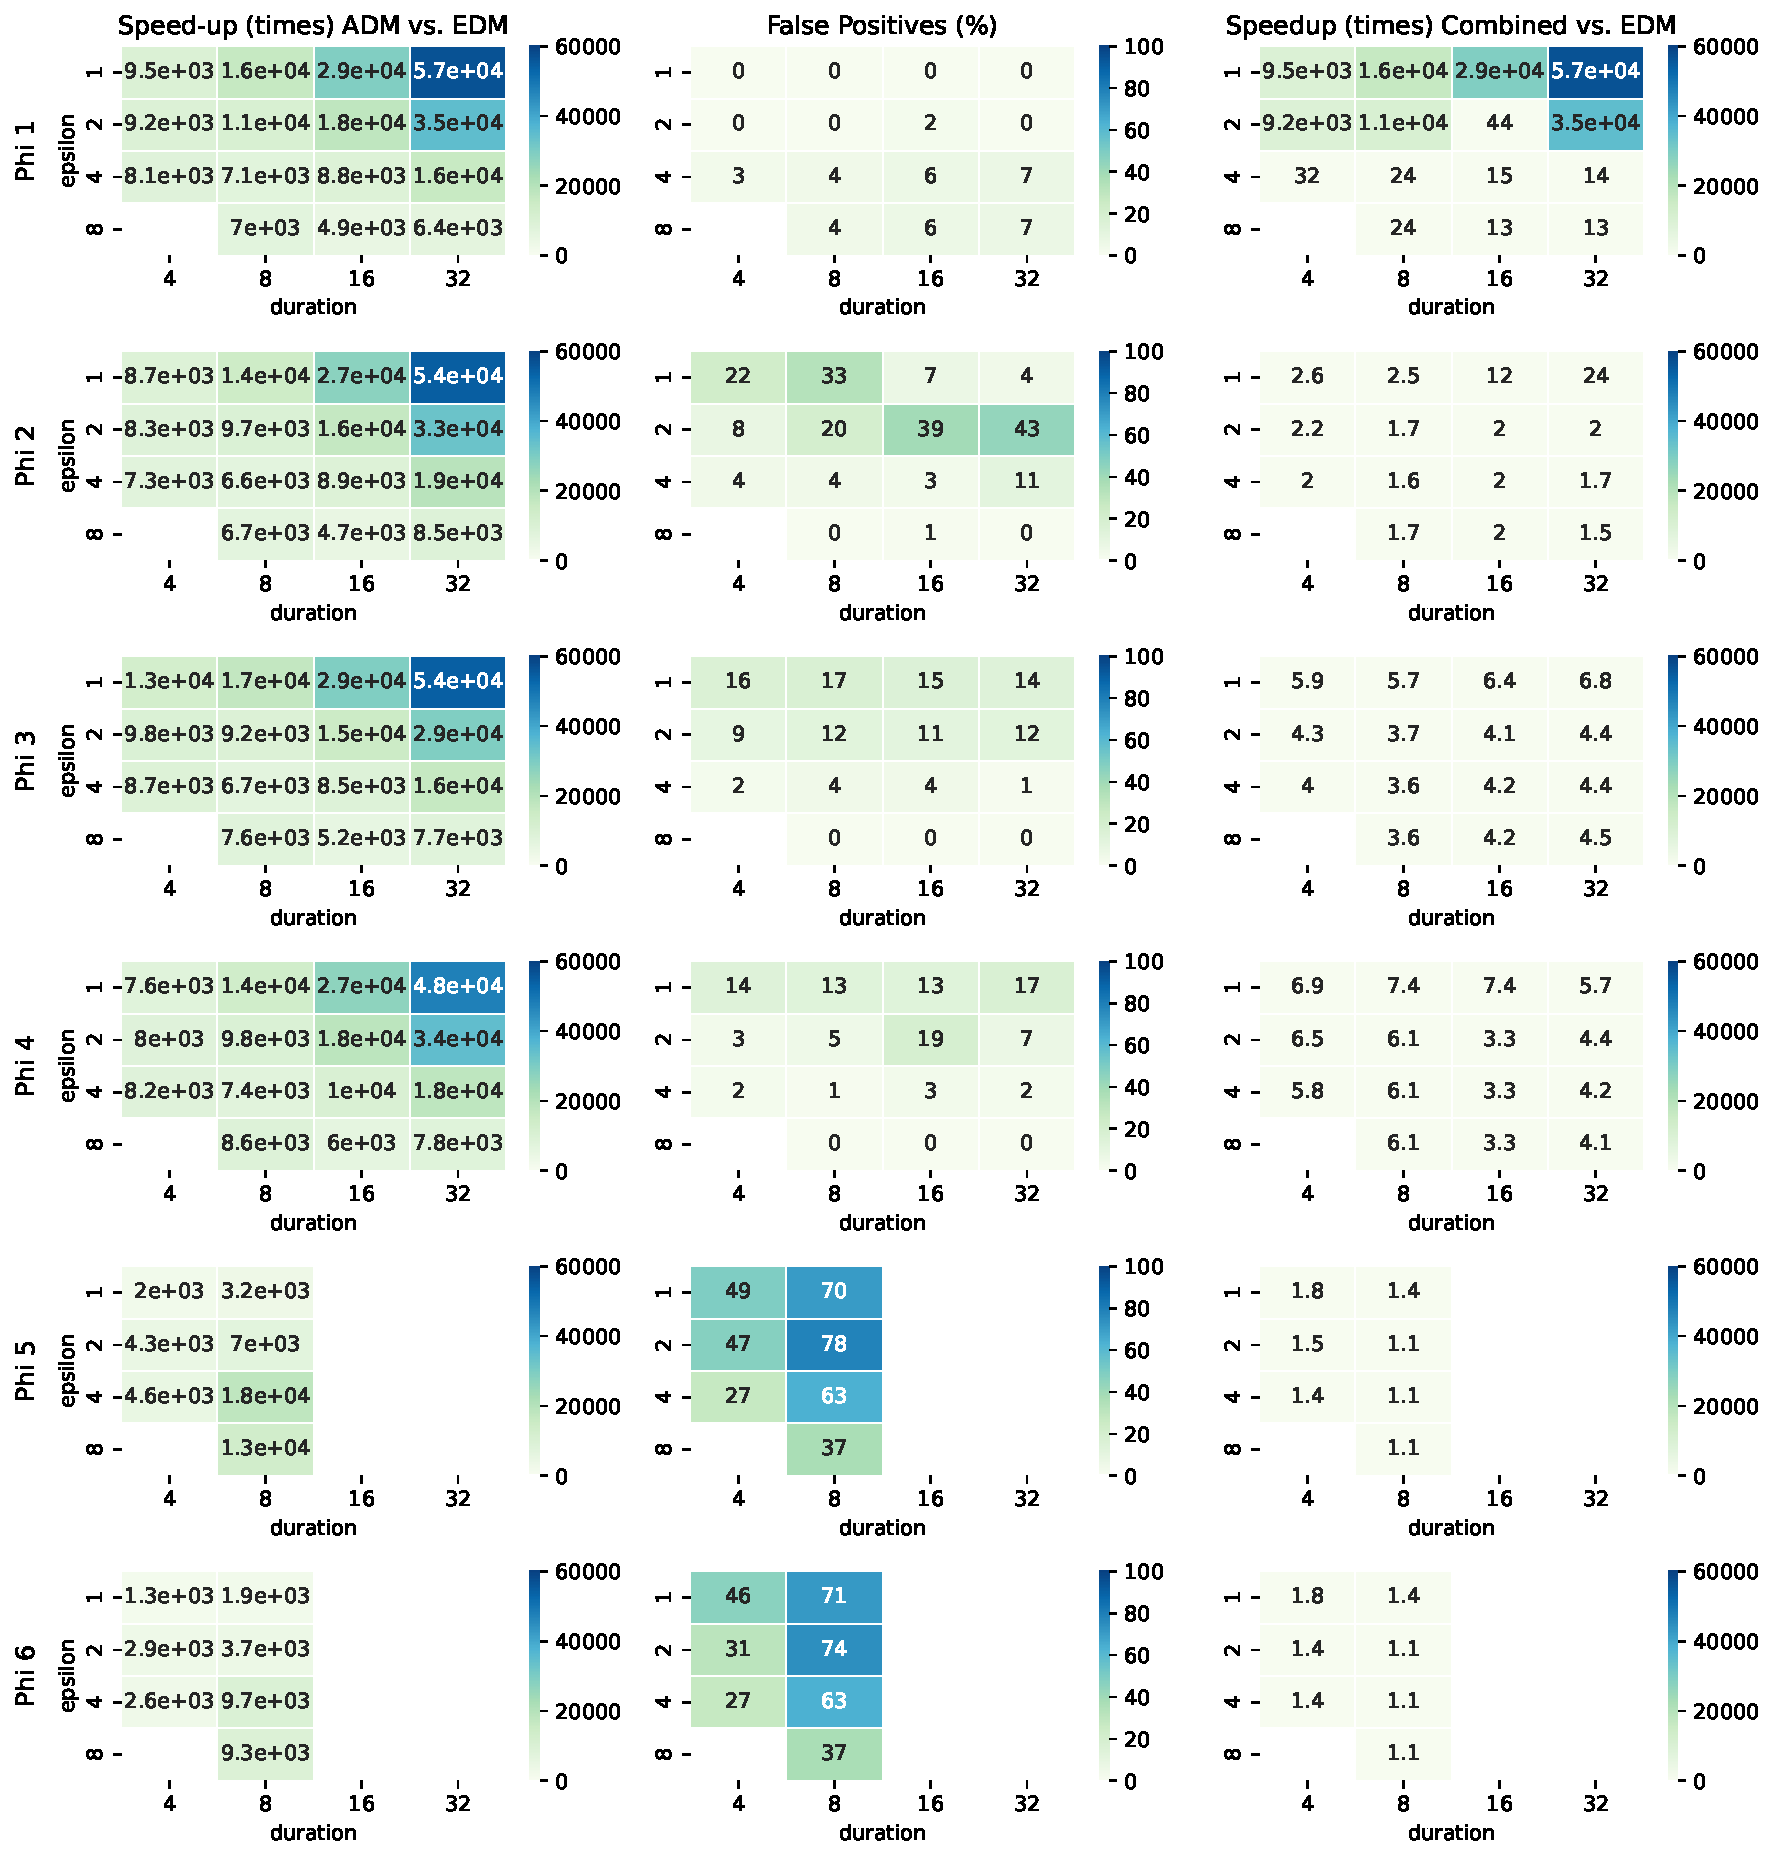
\includegraphics[width=\linewidth]{speedup_all}
			\caption{Results on offline monitoring $\varphi_{1}$ to $\varphi_{6}$ on distributed traces created by the RG.}
			\label{fig:rgresults}
		\end{center}
		%\vspace{1em}
	\end{figure*}
	\clearpage
	\begin{figure*}[p]
		\begin{center}
			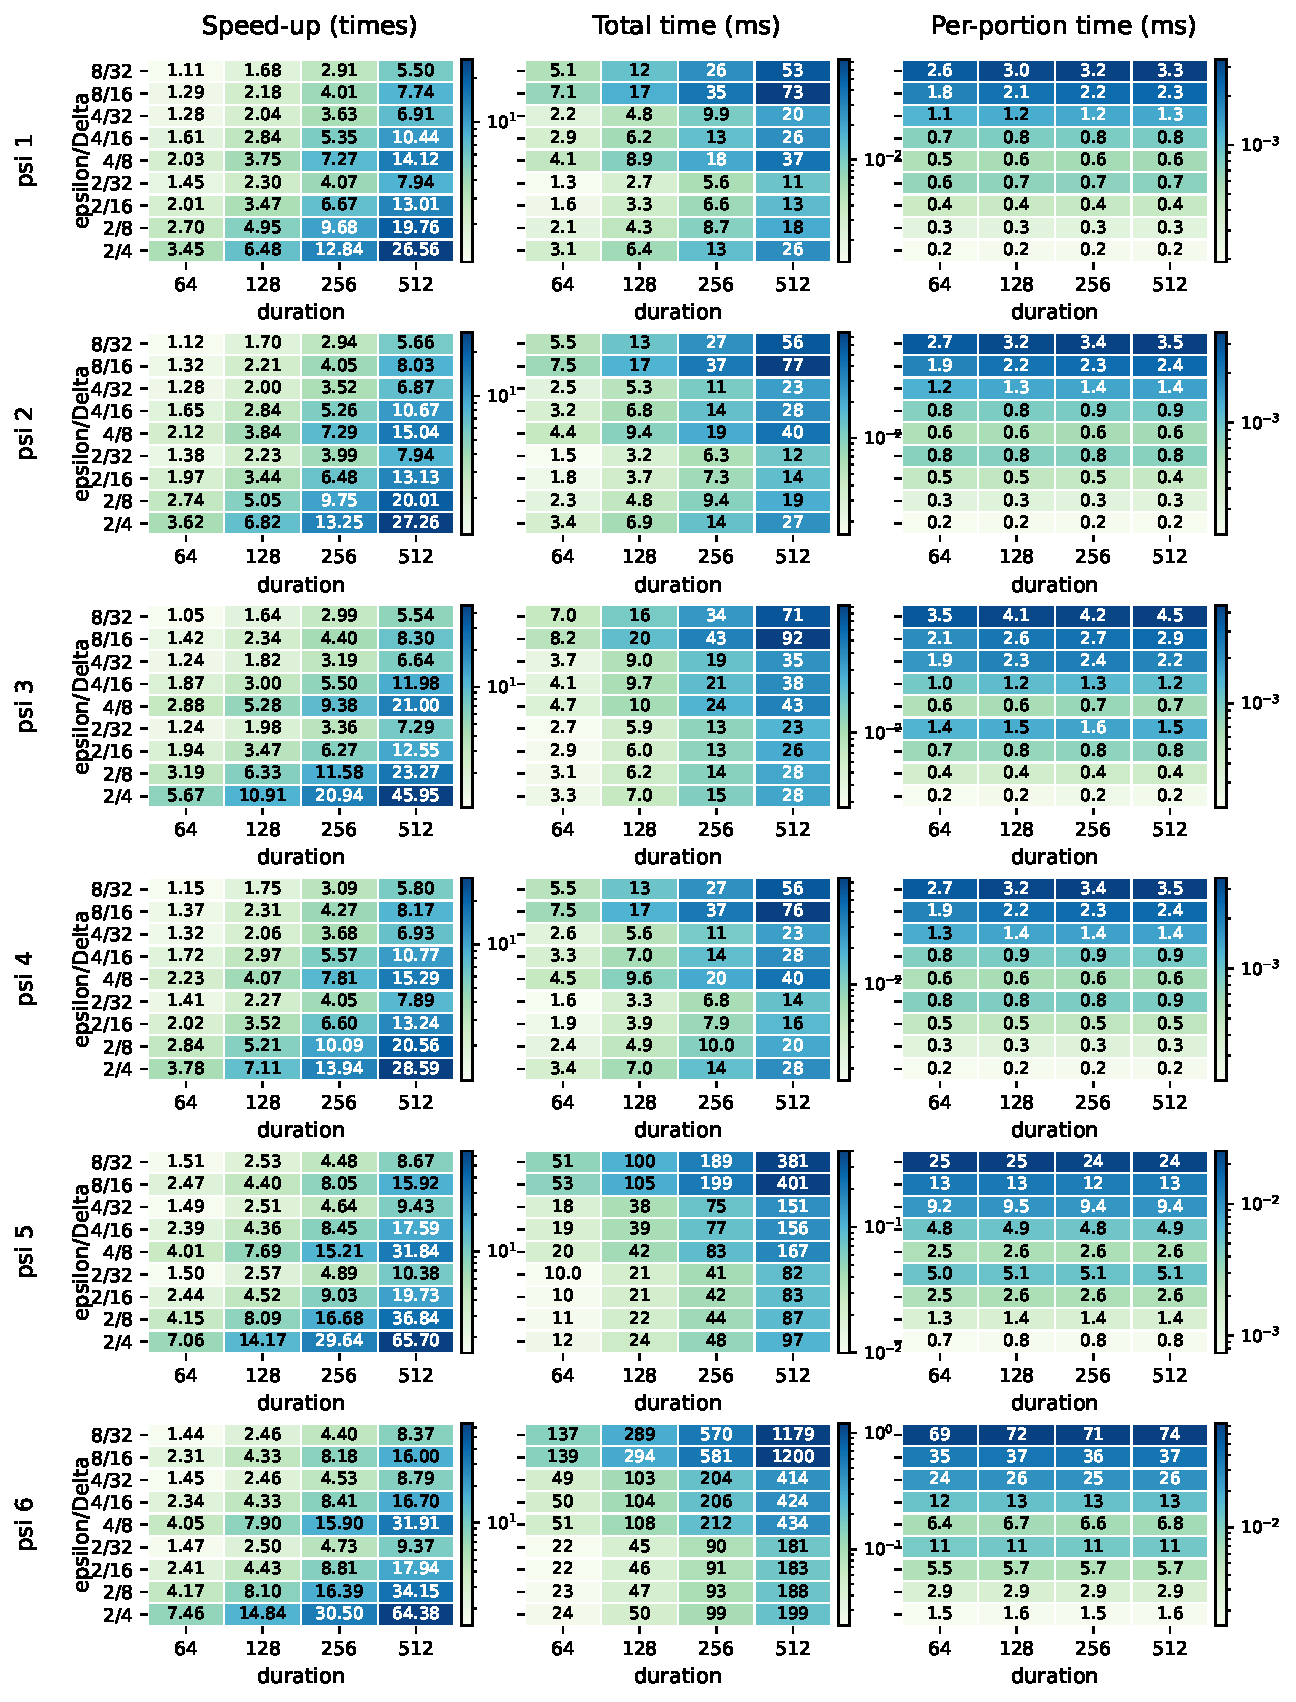
\includegraphics[width=\linewidth]{speedupOnline_all.pdf}
			\caption{Results on online monitoring $\psi_1$ to $\psi_6$ on distributed traces created by the RG.}	\label{fig:rgresultsOnline}
		\end{center}
		%\vspace{1em}
	\end{figure*}
	\clearpage
	\begin{figure*}[t]
		\begin{center}
			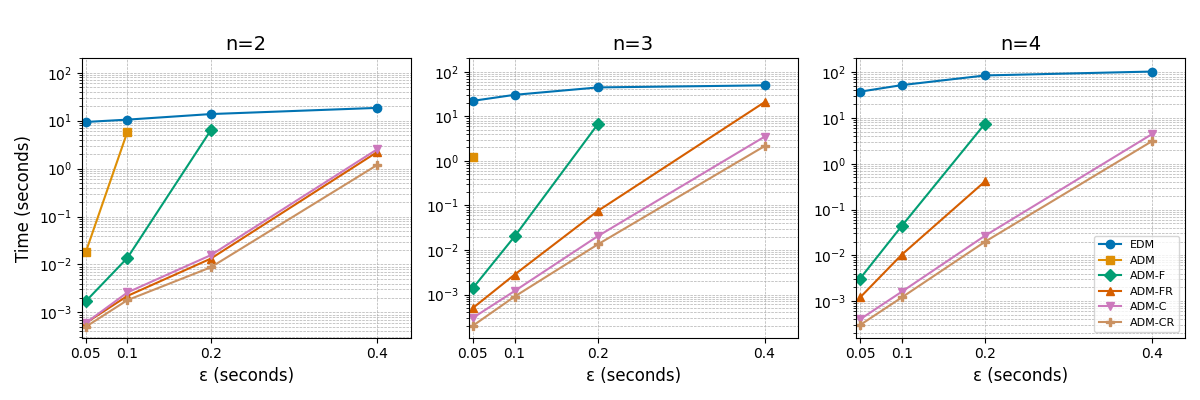
\includegraphics[width=\linewidth]{wt_newnames.png}
			\caption{Running times for monitoring $\varphi_{\text{WT}}$ in log scale. Time limit is 120s, and timed-out instances are not shown.}
			%		\vspace{3mm}
		\end{center}
		%	\vspace{-1em}
	\end{figure*}
	\begin{figure*}[t]
		\begin{center}
			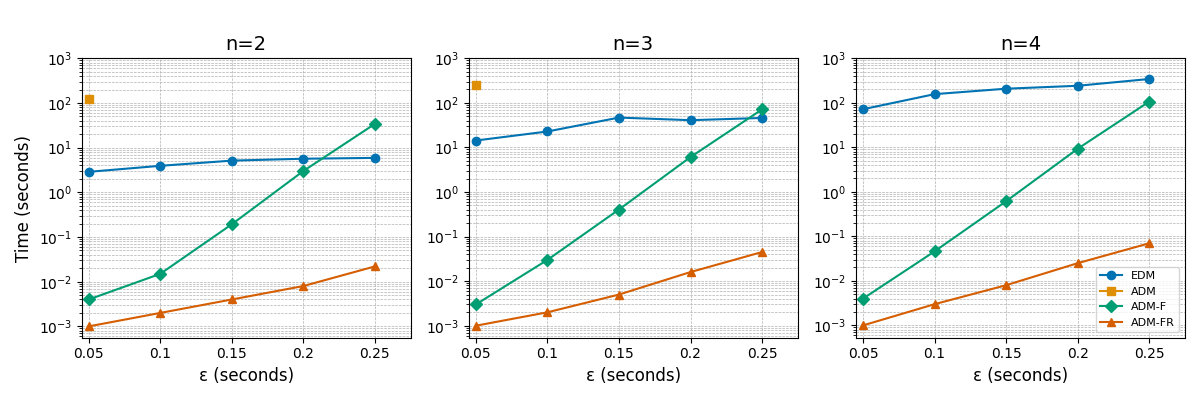
\includegraphics[width=\linewidth]{ms_newnames.png}
			\caption{Running times for monitoring $\varphi_{\text{SD}}$ in log scale. Time limit is 360s, and timed-out instances are not shown.}
		\end{center}
	\end{figure*}
	\clearpage
	
	\bibliographystyle{plain}
	\bibliography{main}
%	\newpage
%	\input appendix
\end{document}